\documentclass[a4paper,12pt]{article}
\input{packages}

\begin{document}


\documentclass[a4paper,12pt]{article}

\input{packages}

\begin{document}

\begin{titlepage}
    \begin{center}
        
        \Huge
        \textbf{La Géométrie euclidienne}
        
        \vspace{0.5cm}
        \large
        Diego Rindisbacher et Océane Patiny
        
        
         \vspace{3cm}
          \includegraphics[scale=2.5]{Euclide.jpg}
          
         \vspace{0.5cm}
          \small
        Gymnase de Renens\\
        Vaud, Suisse\\
        \today
    \end{center}
\end{titlepage}


\end{document}


\documentclass[a4paper,12pt]{article}

\input{packages}

\begin{document}

\abstract{Dans ce document, nous abordons la base de la géométrie euclidienne: des axiomes aux théorèmes.}

\tableofcontents

\pagebreak
\section{Introduction}
Dans ce document, nous allons aborder les bases de la géométrie euclidienne en présentant les axiomes et certains théorèmes. Le mot géométrie provient du grec \textit{géo} - la terre et de \textit{métrie} - la mesure, à l'origine ce serait donc la mesure de ce qui fait partie de la terre.  La géométrie euclidienne étudie les figures et les mesures dans le plan et l'espace. A la base de cette géométrie se trouvent cinq axiomes et des définitions, qui sont tout ce que l'on a pour démontrer de plus en plus d'éléments, qui peuvent nous paraître triviaux tant ils sont omniprésents, mais qu'il a fallu démontrer.

\end{document}

\documentclass[a4paper,12pt]{article}

\input{../../packages}

\begin{document}

\section{Courte biographie d'Euclide}

\begin{figure}[H]
    \centering
    \includegraphics[scale=0.2]{portrait.png}
\end{figure}
Euclide est un mathématicien grec ayant vécu aux alentours de 300 avant J.C.. Il n'y a que très peu d'information à son sujet si ce n'est qu'il a enseigné au musée d'Alexandrie sous Ptolémée $1^{er}$. Euclide ne fut sûrement pas le premier à s'être intéressé à la géométrie, mais la raison pour laquelle on l'appelle le père de la géométrie est "Les éléments d'Euclide". Cet écrit mathématique et géométrique est constitué de treize volumes, qui traitent des fondements de la géométrie euclidienne: des axiomes aux théorèmes et leurs démonstrations. Grâce à la simplicité et la logique de ce recueil, il a été utilisé comme livre de référence durant des siècles.

\end{document}


\documentclass[a4paper,12pt]{article}

\input{packages}

\begin{document}

\section{Définition de la géométrie euclidienne}
La géométrie euclidienne et le regroupement des connaissances géométrique à l'époque d'Euclide et une théorisation des connaissances de façon mathématique. En réalité, il est difficile de définir la géométrie euclidienne, car c'est celle qui nous entoure toujours, et que l'on utilise le plus fréquemment. Pourtant, il est important de la définir car il existe de nombreuses autres géométries, par exemple la géométrie non euclidienne. Celle-ci ne se base pas sur les même axiomes et est donc complètement différente.


\end{document}



\input{definitions/definitions}

\documentclass[a4paper,12pt]{article}

\input{packages}

\begin{document}

\pagebreak
\section{Les axiomes}
\begin{definition}{Axiome:}
 Un axiome est une proposition admise comme un élément de base d'une théorie mathématique et qui est indémontrable en tant que tel.
\end{definition}

Dans cette section, nous allons définir cinq axiomes, qui nous seront indispensables afin de démontrer des théorèmes par la suite.

\subsection{Axiomes de report (axiomes I et II)}
Le transport des segments et des angles ne change pas leur mesure.

\subsection{Cas d'isométrie des triangles (axiome III)}
Il y a trois cas d'isométrie du triangle. On dit que deux triangles sont isométriques lorsqu'ils sont en tous point semblable, longueurs et angles. Afin de démontrer les deux autres cas d'isométrie des triangles, il faut en prendre un comme axiome.\\

\begin{figure}[H]
    \centering
    \includegraphics[scale=0.6]{axiomes/Cas_1.PNG}
  \end{figure}  
\textbf{Premier cas:} Deux triangles qui ont respectivement un angle et les côtés adjacents isométriques sont isométriques.


\subsection{Axiome de continuité (axiome IV)}
Tout nombre réel positif est la longueur d'un segment. Par exemple, pi peut être représenté comme la moitié du périmètre d'un cercle de rayon 1.
\begin{figure}[H]
    \centerline{\includegraphics[scale=0.4]{axiomes/pi.png}}
    \label{fig:fig2}
\end{figure}

\pagebreak
Ou alors, on peut représenter la racine de deux comme l'hypothénuse d'un triangle rectangle dont les deux côtés valent 1.
\begin{figure}[H]
    \centering
    \includegraphics[scale=0.6]{axiomes/racine2.png}
\end{figure}



\subsection{Axiome des parallèles (axiome V)}
Pour un point donné, il existe une et une seule droite parallèle à une droite et passant par ce point.
\begin{figure}[H]
    \centering
    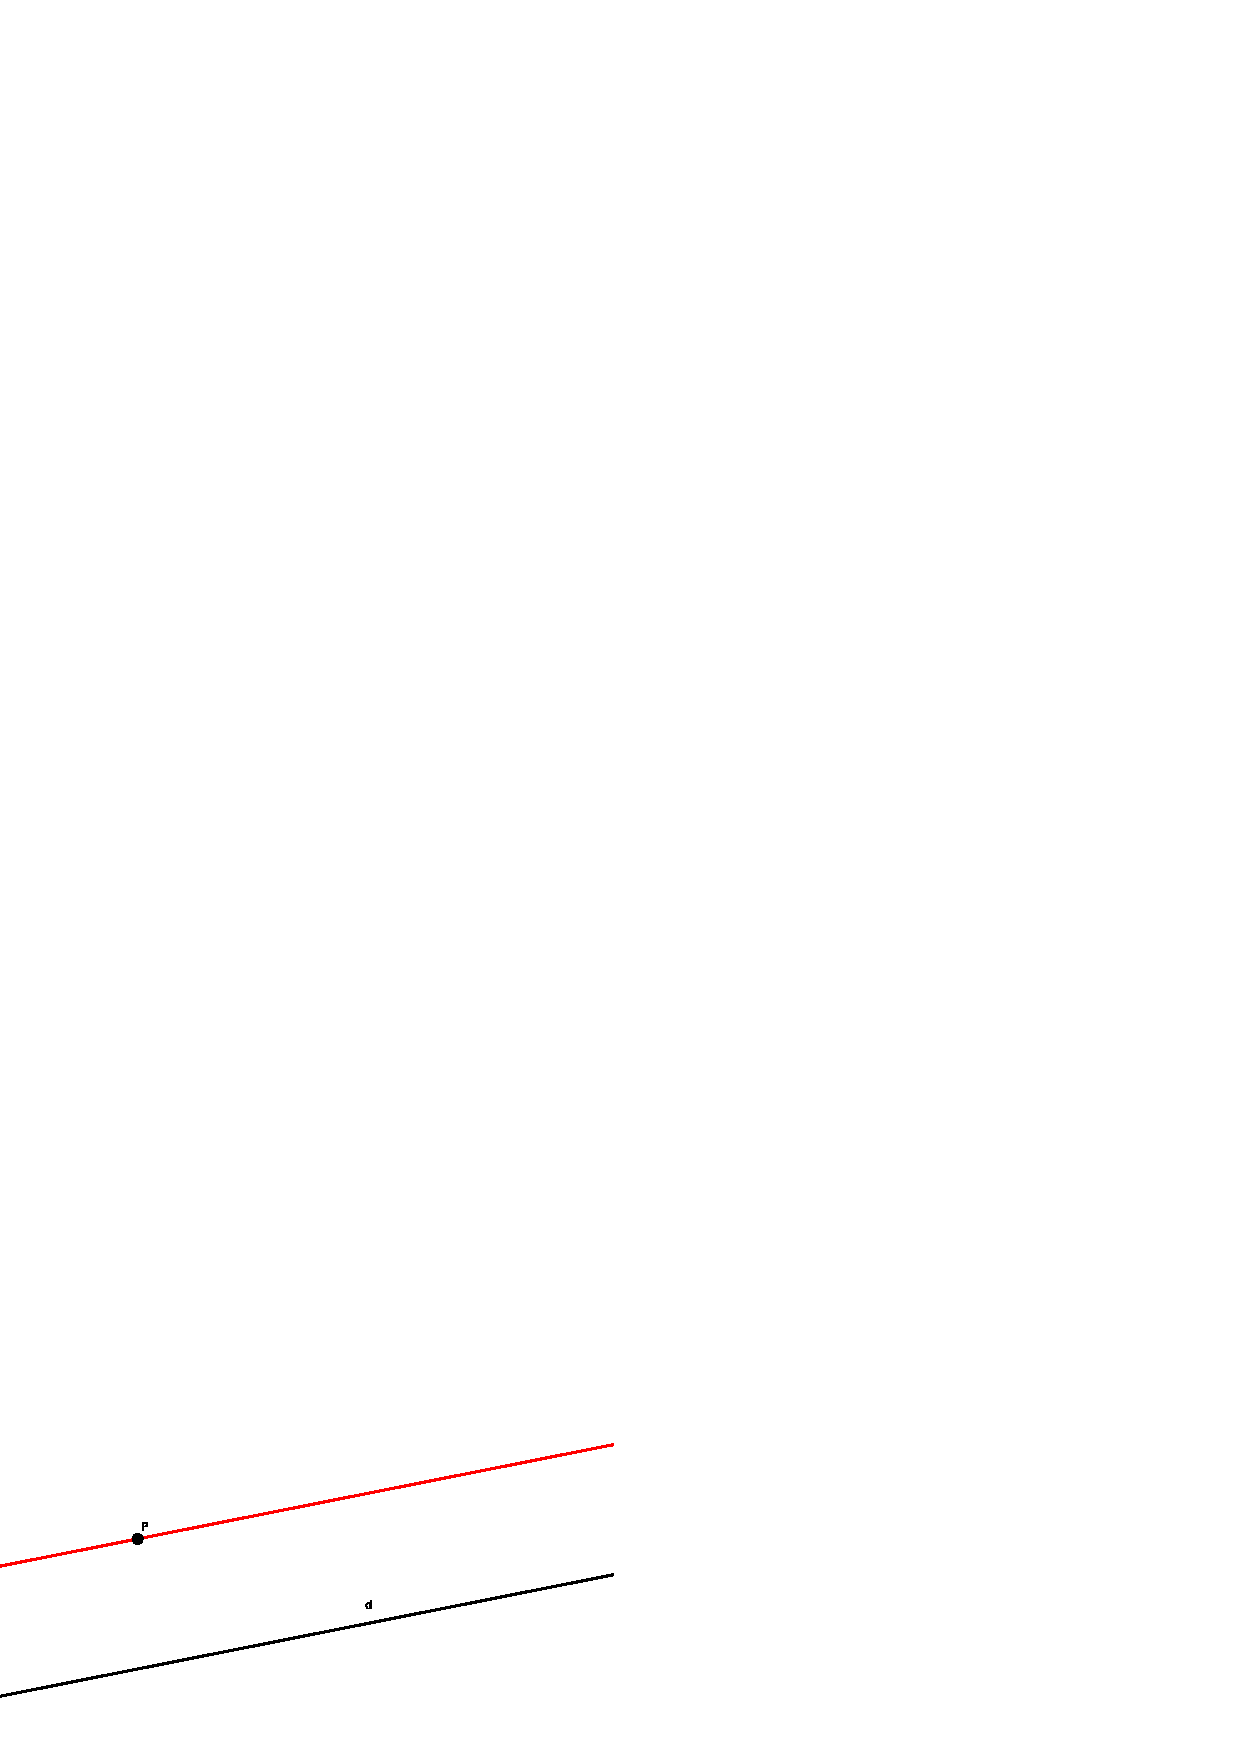
\includegraphics[scale=0.6]{axiomes/parallel.png}
\end{figure}


\end{document}



\pagebreak
\section{Théorèmes}
Dans cette partie, nous allons démontrer plusieurs théorèmes en ne se basant que sur ce que l'on sait déjà, c'est-à-dire les cinq axiomes.

\documentclass[a4paper,12pt]{article}

\input{../../packages}

\begin{document}

\subsection{Théorème de l'angle externe}
\begin{theorem}
Dans tout triangle et pour chaque sommet, l'angle externe est plus grand que l'angle intérieur en chacun des autres sommets.
\end{theorem}

\begin{proof}
Considérons un triangle $\triangle abc$ qui a $\alpha'$ comme angle externe à $\alpha$.
\begin{figure}[H]
    \centering
    \includegraphics[scale=0.9]{Angle_externe_1.PNG}
\end{figure}

Se présentent alors trois cas possibles :

\begin{enumerate}
    \item $\alpha'  \equiv \gamma$
    \item $\alpha' < \gamma$
    \item $\alpha' > \gamma$
\end{enumerate}
Il nous faut démontrer que les cas 1 et 2 sont impossibles et que seul le cas 3 reste correct.
\begin{enumerate}

    \item Tout d'abord nous reportons le côté $CB$ sur le prolongement du segment $AB$ et obtenons le segment DA. Ensuite, nous relions les points $C$ et $D$. Ainsi nous obtenons un nouveau triangle $\triangle DCA$, dont l'un des angles est $\alpha'$.
	Grâce au premier cas d'isométrie des triangles, on déduit que les triangles $\triangle DCA$ et $\triangle abc$ sont isométriques ($DA \equiv CB$, $\alpha'\equiv \gamma$ et $CA$ est commun aux deux triangles). 
	Par conséquent $\angle{DCA}$ équivaut à alpha. Ce qui signifie que l'angle $BCD$ ($\alpha + \gamma$) est plat, donc que les triangles sont plats.
	Ce qui est absurde, $\alpha'$ ne peut pas être équivalent à $\gamma$. 
    \begin{figure}[H]
        \centering
        \includegraphics[scale=0.6]{Angle_externe_2.png}
    \end{figure}
	\begin{flushright}
    $\bigstar $
    \end{flushright}
    
    \item Nous considérons le triangle $\triangle abc$ et nous plaçons un point $B'$ sur le segment $AB$, tel que $\angle{ACB'} \equiv \alpha'$.
     Donc ce triangle a un angle externe équivalent à un angle interne, ce qui nous renvoie au premier cas. 
     Il n'est donc pas possible que $\alpha'$ soit plus petit que $\gamma$.
     \begin{figure}[H]
    \centering
    \includegraphics[scale=0.9]{Angle_externe_3.PNG}
\end{figure}
     \begin{flushright}
    $\bigstar $
    \end{flushright}

\end{enumerate}

Nous avons démontré que les cas 1 et 2 sont impossibles et que la seule possibilité est que $\alpha' > \gamma$.
\end{proof}


\end{document}


\documentclass[a4paper,12pt]{article}

\input{packages}

\begin{document}

\pagebreak
\subsection{Deuxième cas d'isométrie des triangles}
\begin{theorem}
Deux triangles qui ont respectivement un côté et les angles adjacents isométriques sont isométriques.
\end{theorem}
\begin{hyp}
$a_1 \equiv a_2$, $\beta_1 \equiv \beta_2$ et $\gamma_1 \equiv \gamma_2$
\end{hyp}
\begin{concl}
$b_1 \equiv b_2$, $c_1 \equiv c_2$ et que $\alpha_1 \equiv \alpha_2$
\end{concl}
\begin{proof}
Considérons deux triangles $\triangle a_1b_1c_1$ et $\triangle a_2b_2c_2$. Nous avons reporté le côté $c_2$ sur le côté $c_1$. alors, il y a trois possibilités:
\begin{figure}[H]
    \centering
    \includegraphics[scale=0.45]{theorems/isom2/cas2.png}
\end{figure}
\begin{enumerate}
\item $c_1 = c_2$, alors les deux triangles sont isométriques (axiome III)
\item $c_1<c_2$
\item $c_1>c_2$
\end{enumerate}

\pagebreak
Dans le deuxième et troisième cas, on forme le triangle $\triangle b_1b_3c_2'$. Ce triangle est isométrique au triangle $\triangle a_2b_2c_2$, car ils ont en commun un angle compris entre deux côtés isométriques. Par conséquent, $\gamma_2\equiv \gamma_3$, donc $\gamma_1$ et $\gamma_3$ sont confondus, d est nul et $c_1\equiv c_2$. On en revient donc au premier cas: les deux triangles $\triangle a_1b_1c_1$ et $\triangle a_2b_2c_2$ sont isométriques grâce au premier cas d'isométrie des triangles.


\begin{figure}[H]
    \centering
    \includegraphics[scale=0.6]{theorems/isom2/Cas2_2.png}
\end{figure}



\end{proof}

\end{document}


\documentclass[a4paper,12pt]{article}

\input{packages}

\begin{document}

\pagebreak
\begin{corollary}
Deux triangles qui ont respectivement un côté et deux angles isométriques sont isométriques.
\end{corollary}

\begin{proof}
Considérons deux triangles $\triangle a_1b_1c_1$ et $\triangle a_2b_2c_2$.

\begin{figure}[H]
    \centering
    \includegraphics[scale=0.5]{theorems/corIsom2/corIsom2.png}
\end{figure}

\begin{hyp}
$a \equiv a'$, $\beta \equiv \beta'$ et $\alpha \equiv \alpha'$
\end{hyp}
\begin{concl}
$b \equiv b'$, $c \equiv c'$ et  $\gamma \equiv \gamma'$
\end{concl}

Pour démontrer ce corollaire, nous avons superposé ces deux triangles. Il existe alors trois cas possibles:
\begin{enumerate}
    \item $c_1 \equiv c_2$
    \item $c_1 > c_2$
    \item $c_1 < c_2$
\end{enumerate}
Dans le premier cas, comme $c_1 \equiv c_2$, $\beta_1 \equiv \beta_2$ et $a_1 \equiv a_2$, on sait que les deux triangles sont isométriques (axiome III).\\
Dans les deux autres cas, on peut observer la formation du triangle $b_1b_2'c_3$, dont l'un des angles est alpha 1. Considérons ce triangle, on peut observer que l'un de ses angles externes (voir sous-section 6.1) est $\alpha_2$, ce qui implique que $\alpha_1 < \alpha_2$, ce qui est absurde. Le seul cas possible est donc le premier.
\begin{figure}[H]
    \centering
    \includegraphics[scale=0.6]{theorems/corIsom2/corIsom2_2.png}
\end{figure}
\end{proof}

\begin{remark}
Un corollaire est une démonstration nouvelle que l'on peut faire grâce à une affirmation précédente. Le mot provient du latin "corollarium", qui signifie littéralement "petite couronne".\footnote{CNRTL, dictionnaire étymologique, http://www.cnrtl.fr/}
\end{remark}

\end{document}


\documentclass[a4paper,12pt]{article}

\input{packages}

\begin{document}

\pagebreak
\subsection{Triangles isocèles}
\begin{theorem}
Un triangle est isocèle si et seulement si les angles opposés aux côtés isométriques sont isométriques.
\end{theorem}

\begin{proof}
La démonstration de ce théorème se déroule en deux parties:
\begin{itemize}
    \item La première partie doit démontrer qu'un triangle avec deux côtés isométriques est isocèle
    \item La deuxième partie doit démontrer qu'un triangle avec deux angles isométriques est isocèle
    \end{itemize}

    \begin{enumerate}
        \item Nous considérons le triangle $ABC$.
        \begin{figure}[H]
        \centering
        \includegraphics[scale=0.7]{schema/iso1.png}
    \end{figure}
    
    
    \begin{hyp}
    $a\equiv b$
    \end{hyp}
    \begin{concl}
    $\alpha \equiv \beta$
    \end{concl}
    En faisant la bissectrice B de l'angle $\gamma$, nous obtenons deux triangles (1 et 2) qui ont un angle isométrique ($\gamma_1 \equiv \gamma_2$) compris entre deux côtés isométriques ($a\equiv b$, B). Donc nous savons que les triangles 1 et 2 sont isométriques, grâce au premier cas d'isométrie des triangles. Par conséquant, $\alpha \equiv \beta$ et le triangle $ABC$ est isocèle.
    
    
    \begin{figure}[H]
        \centering
        \includegraphics[scale=0.45]{schema/iso2.png}
    \end{figure}
    
    
    
    
    \item Nous considérons le triangle $ABC$.
    \begin{figure}[H]
            \centering
            \includegraphics[scale=0.7]{schema/iso3.png}
    \end{figure}

    \begin{hyp}
     $\alpha \equiv \beta$
    \end{hyp}
    \begin{concl}
     $a\equiv b$
    \end{concl}
    Nous tirons la hauteur h partant de $\gamma$ et obtenons deux triangles 1 et 2. Ces deux triangles ont deux angles ($\alpha \equiv \beta$, les angles droits) et un côté (h) isométriques, donc ils sont isométriques (corollaire du deuxième cas d'isométrie des triangles). Par conséquent $a\equiv b$ et le triangle $ABC$ est isocèle.
    
    \begin{figure}[H]
        \centering
        \includegraphics[scale=0.45]{schema/iso4.png}
    \end{figure}
    
\end{enumerate}
\end{proof}

\end{document}

\documentclass[a4paper,12pt]{article}

\input{packages}

\begin{document}


\pagebreak
\subsection{Propriétés des bissectrices}
\begin{theorem}
La bissectrice d'un angle est le lieu géométrique des points intérieurs à l'angle et équidistants à ses côtés.
\end{theorem}
Le théorème implique deux choses:
\begin{enumerate}
\item Un point qui se trouve sur la bissectrice d'un angle est équidistant à ses côtés
\item Un point équidistant au côtés d'un angle se trouve sur sa bissectrice
\end{enumerate}
\begin{proof}
Nous considérons deux droites $d$ et $d'$ qui se coupent en un point $A$, on trace la bissectrice de l'angle en $A$ et on obtient deux angles $\alpha$ et $\alpha'$. Puis nous traçons deux segments $a$ et $a'$ qui partent d'un point $Q$ sur la bissectrice et qui coupent les droites $d$ et $d'$ perpendiculairement, aux points $D$ et $D'$.
\begin{figure}[H]
    \centering
    \includegraphics[scale=0.8]{schema/Bissectrices_1.PNG}
\end{figure}


\begin{hyp}
$d$ et $d'$sont deux droites sécantes, $\alpha \equiv \alpha'$, $a\perp d$, $a' \perp d'$
\end{hyp}
\begin{concl}
$a\equiv a'$
\end{concl}
En faisant la construction, nous obtenons deux triangles $\triangle AQD$ et $\triangle A'QD'$. Comme ces deux triangles partagent un côté et ont deux angles isométriques ($\alpha \equiv \alpha'$, les angles droits), ils sont isométriques (corollaire du deuxième cas d'isométrie des triangles). Donc $a \equiv a'$.
\end{proof}

\begin{proof}
Nous considérons deux droites $d$ et $d'$ qui se coupent en un point $A$. Puis nous considérons un point $Q$ qui est à égale distance de $d$ et $d'$. Ensuite nous traçons deux segments $a$ et $a'$ qui coupent les droites $d$ et $d'$ perpendiculairement aux points $D$ et $D'$ et qui passent par $Q$. En reliant le point Q et le point A, nous obtenons deux angles $\alpha$ et $\alpha'$.

 \begin{figure}[H]
    \centering
    \includegraphics[scale=0.8]{schema/Bissectrices_3.PNG}
\end{figure}


\begin{hyp}
$d$ et $d'$sont deux droites sécantes, $a\equiv a'$, $a\perp d$, $a' \perp d'$
\end{hyp}
\begin{concl}
$\alpha \equiv \alpha'$
\end{concl}
Ainsi, nous obtenons deux triangle $\triangle AQD$ et $\triangle A'QD'$. Pour le moment, nous savons que ces deux triangles ont un côté en commun et un angle isométrique. Pour trouver une troisième grandeur isométrique, nous formons le triangle $\triangle DD'Q$. Ce triangle est isocèle, parce que $a\equiv a'$. Donc le triangle $\triangle DD'A$ l'est aussi et les distances $AD'$ et $AD$ sont isométriques. 

 \begin{figure}[H]
    \centering
    \includegraphics[scale=0.8]{schema/Bissecrtices_4.PNG}
\end{figure}


Donc, grâce au corollaire du deuxième cas d'isométrie, nous savons que les triangle $\triangle AQD$ et $\triangle A'QD'$ sont isométriques. Par conséquent, $\alpha \equiv \alpha'$.
\end{proof}

\end{document}

\documentclass[a4paper,12pt]{article}

\input{packages}

\begin{document}

\pagebreak
\subsection{Troisième cas d'isométrie des triangles}
\begin{theorem}
Deux triangles qui ont respectivement les trois côtés isométriques sont isométriques.
\end{theorem}
\begin{proof}
Nous considérons deux triangles $a_1b_1c_1$ et $a_2b_2c_2$.

\begin{figure}[H]
    \centering
    \includegraphics[scale=0.6]{theorems/isom3/Cas_3.PNG}
\end{figure}

 \begin{hyp}
     $a_1\equiv a_2$,
     $b_1\equiv b_2$ et
     $c_1\equiv c_2$
 \end{hyp}
 \begin{concl}
     $\alpha \equiv \alpha'$,
     $\beta \equiv \beta'$ et
     $\gamma \equiv \gamma'$
 \end{concl}
 Nous rassemblons les deux triangles en un quadrilatère en superposant $c_1$ et $c_2$. 
 
 \begin{figure}[H]
    \centering
    \includegraphics[scale=0.6]{theorems/isom3/Cas3_2.png}
\end{figure}
 
 Puis nous relions les sommets en $\gamma$ et $\gamma'$, nous nommons ce segment $h$. Ainsi, nous obtenons deux triangles qui sont isocèles $\triangle a_1a_2h$ et $\triangle b_1b_2h$ ($a_1\equiv a_2$ pour $\triangle a_1a_2h$ et $b_1\equiv b_2$ pour $\triangle b_1b_2h$, voir section 6.3) ce qui signifie que $\theta_1 \equiv \theta_2$ et que $\theta_3 \equiv \theta_4$.
 
 
 \begin{figure}[H]
    \centering
    \includegraphics[scale=0.6]{theorems/isom3/Cas3_3.png}
\end{figure}

 
 
 Finalement, comme $\alpha \equiv \theta_1 + \theta_2$ et $\alpha' \equiv \theta_3 + \theta_4$, nous avons démontré que $\alpha \equiv \alpha'$. Les deux triangles $a_1b_1c_1$ et $a_2b_2c_2$ sont donc isométriques (axiome III).
\end{proof}

\end{document}


\documentclass[a4paper,12pt]{article}

\input{packages}

\begin{document}

\pagebreak
\subsection{Cosinus de la différence de deux angles}
\begin{theorem}
Le cosinus de la différence de deux angles est égal à la somme du produit de leurs sinus et du produit de leurs cosinus.
\begin{equation}
    cos(\beta-\alpha) = cos \alpha \cdot cos \beta + sin \alpha \cdot sin \beta
\end{equation}
\end{theorem}
\begin{figure}[H]
    \centering
    \includegraphics[scale=0.8]{theorems/cosinus/diff.PNG}
\end{figure}

\begin{proof}
Nous considérons le cercle trigonométrique suivant, dans lequel nous avons représenté l'angle $\beta-\alpha$, que nous avons reporté sur l'axe du cosinus (grâce à l'axiome de report). Ainsi, en reliant les points QP et les points AR, nous obtenons deux triangles ayant un angle isométrique compris entre deux côtés isométriques. Ce qui signifie que les triangles $\Delta ARO$ et $\Delta PQO$ sont isométriques (axiome III). Donc, on peut écrire que:
\begin{equation}
    ||\vec{PQ}|| \equiv ||\vec{AR}||
\end{equation}

On connait aussi les coordonnées des quatre points P, Q, A et R, qui sont:
\begin{equation}
\begin{split}
   & P = (cos \beta, sin \beta)\\
   & Q = (cos \alpha, sin \alpha)\\
   & A = (1, 0)\\
   & R = (cos (\beta-\alpha), sin (\beta-\alpha))
\end{split}
\end{equation}

Donc, on peut décrire les vecteurs $\vec{PQ}$ et $\vec{AR}$ de la manière suivante:

\begin{equation}
\begin{split}
 & \vec{PQ} = \binom{cos\alpha-cos\beta}{sin\alpha-sin\beta} \rightarrow ||\vec{PQ}|| = \sqrt{(cos\alpha-cos\beta)^2 + (sin\alpha-sin\beta)^2}\\
 & \vec{AR} = \binom{cos(\beta-\alpha)-1}{sin(\beta-\alpha)} \rightarrow ||\vec{AR}|| = \sqrt{(cos(\beta-\alpha)-1)^2 + (sin(\beta-\alpha)^2}
\end{split}
\end{equation}

Finalement, comme $||\vec{PQ}||$ et $||\vec{AR}||$ sont équivalents, on peut écrire l'égalité suivante:
\begin{equation}
(cos(\beta-\alpha)-1)^2 + (sin(\beta-\alpha)^2 = (cos\alpha-cos\beta)^2 + (sin\alpha-sin\beta)^2
\end{equation}
Ce qui développé donne:
\begin{equation}
2-2cos(\beta-\alpha) = 2-2(cos \alpha \cdot cos \beta + sin \alpha \cdot sin \beta)
\end{equation}
Nous avons donc démontré la formule du cosinus de la différence de deux angles:
\begin{equation*}
    cos(\beta-\alpha) = cos \alpha \cdot cos \beta + sin \alpha \cdot sin \beta
\end{equation*}
\end{proof}

\end{document}


\documentclass[a4paper,12pt]{article}

\input{packages}

\begin{document}

\pagebreak
\subsection{Isométrie de deux angles opposés par le sommet}
\begin{theorem}
Deux angles opposés par le sommet sont isométriques.
\end{theorem}
\begin{proof}
Nous considérons deux droites sécantes.

 \begin{figure}[H]
    \centering
    \includegraphics[scale=0.8]{schema/anglesym.PNG}
\end{figure}


\begin{hyp}
     Deux droites se croisent en un point
 \end{hyp}
 \begin{concl}
     $\alpha \equiv \beta$, $\gamma$ est l'angle complémentaire de $\alpha$ et $\beta$
 \end{concl}
 Comme $\gamma$ est l'angle complémentaire de $\alpha$ et $\beta$, on peut écrire l'équation suivante:
 \begin{equation}
 \gamma + \alpha = 180\degree \rightarrow \alpha = 180\degree-\gamma
 \end{equation}
 \begin{equation}
 \gamma+ \beta = 180\degree \rightarrow \beta = 180\degree-\gamma
 \end{equation}
 Par conséquent, on sait que $\alpha \equiv \beta$.
\end{proof}

\end{document}

\documentclass[a4paper,12pt]{article}

\input{packages}

\begin{document}

\pagebreak
\subsection{Théorème de la transversale}
\begin{theorem}\label{th:transversale}
Si deux droites $d$ et $d'$ ayant $e$ comme transversale ont une paire d'angles alternes-internes, alternes-externes ou correspondant isométriques, alors ces deux droites sont isométriques.\\
Aussi, si l'on considère la transversale $e$ à deux droites $d$ et $d'$ parallèles, alors une paire d'angle est isométrique lorsque ces angles sont: alternes-internes, alternes-externes ou  correspondants.
\end{theorem}
\begin{proof}
Nous considérons deux droites $d$ et $d'$ qui on $e$ comme transversale.
\begin{figure}[H]
    \centering
    \includegraphics[scale=1]{theorems/transversal/Transversale.PNG}
\end{figure}


\begin{hyp}
     $d$, $d'$ et $e$ sont trois droites,
     $\alpha$ et $\alpha'$ sont correspondants et
     $\alpha \equiv \alpha'$
 \end{hyp}
 \begin{concl}
     $d \parallel d'$
 \end{concl}
 En considérant l'hypothèse, il existe deux cas possibles:
 \begin{enumerate}
     \item $d$ et $d'$ se coupent en un point r
     \item $d$ et $d'$ sont parallèles
 \end{enumerate}
 Il nous faut démontrer que le cas 1) est faux et que le deuxième cas est le seul possible.\\
 Supposons que $d$ et $d'$ se coupent en un point r, il y a alors deux cas de figure possibles:
 \begin{enumerate}[label=\emph{\alph*}.]
  \item $\alpha'$ est à l'intérieur du triangle $\triangle pp'r$ et $\alpha$ est un angle externe. Par conséquent, grâce au théorème de l'angle externe, on sait que $\alpha>\alpha'$, ce qui est absurde. Donc il est impossible que d et d' se croisent et que $\alpha$ ou $\alpha'$ soient à l'intérieur du triangle $\triangle pp'r$.
  
    \begin{figure}[H]
        \centering
        \includegraphics[scale=0.5]{theorems/transversal/Transversale_3.png}
    \end{figure}
  
  
  \item Les angles $\alpha$ et $\alpha'$ sont à l'extérieur du triangle $\triangle pp'r$. Dans ce cas-là, par l'isométrie de deux angles opposés par le sommet (sous-section 6.7), on se retrouve dans le même cas qu'en a). Donc $\alpha$ et $\alpha'$ ne peuvent pas être à l'extérieur du triangle $\triangle pp'r$.
  
  
  \begin{figure}[H]
    \centering
    \includegraphics[scale=0.7]{theorems/transversal/Transversale_2.PNG}
\end{figure}

  
 \end{enumerate}
 Le seul cas possible est donc le cas 2, $d$ et $d'$ sont parallèles.
\end{proof}

\begin{proof}
Nous considérons deux droites $d$ et $d'$ qui on $e$ comme transversale.

 \begin{figure}[H]
    \centering
    \includegraphics[scale=0.6]{theorems/transversal/Transversale_4.png}
\end{figure}


\begin{hyp}
     $d$, $d'$ et $e$ sont trois droites,
     $\alpha$ et $\alpha'$ sont correspondants et
     $d \parallel d'$
 \end{hyp}
 \begin{concl}
     $\alpha \equiv \alpha'$
 \end{concl}
 Nous construisons la droite $d''$ qui passe par $p$ en reportant l'angle $\alpha'$. Grâce à la première partie de la démonstration, nous déduisons que d' est parallèle à d''. Donc, comme d' et d'' sont parallèles et qu'elles croisent e au point p, ces deux droites sont confondues (axiome des parallèles). On en conclu que $\alpha \equiv \alpha'$.
\end{proof}

\end{document}


\documentclass[a4paper,12pt]{article}

\input{packages}

\begin{document}

\pagebreak
\subsection{Théorème de la somme des angles d'un triangle}
\begin{theorem}\label{th:180}
La somme des angles d'un triangle équivaut à 180 degrés.
\end{theorem}
\begin{proof}

Nous considérons un triangle $\triangle ABC$, puis nous traçons une parallèle au côté c passant par le sommet C.
\begin{figure}[H]
    \centering
    \includegraphics[scale=0.6]{theorems/sommeAngle/Somme_angles.PNG}
\end{figure}


\begin{hyp}
$\triangle ABC$ est quelconque
\end{hyp}
\begin{concl}
$\alpha + \beta +\gamma = 180 \degree$
\end{concl}
Grâce au théorème des transversales et à l'isométrie de deux angles opposés par le sommet, nous savons que $\alpha + \beta +\gamma = 180 \degree$.
\end{proof}

\end{document}


\documentclass[a4paper,12pt]{article}

\input{packages}

\begin{document}

\subsection{Théorème du segment moyen}
\begin{theorem}
La médiatrice d'un segment est le lieu géométrique des points équidistants à ses extrémités.
\end{theorem}

\end{document}

\documentclass[a4paper,12pt]{article}

\input{packages}

\begin{document}

\pagebreak
\subsection{Théorème des diagonales du parallélogramme}
\begin{theorem}\label{th:parallelogramme}
Les diagonales d'un parallélogramme se coupent en leur milieu.
\end{theorem}

\begin{proof}
Nous considérons un parallélogramme $ABCD$ dont les diagonales se coupent au point $O$.

\begin{figure}[H]
        \centering
        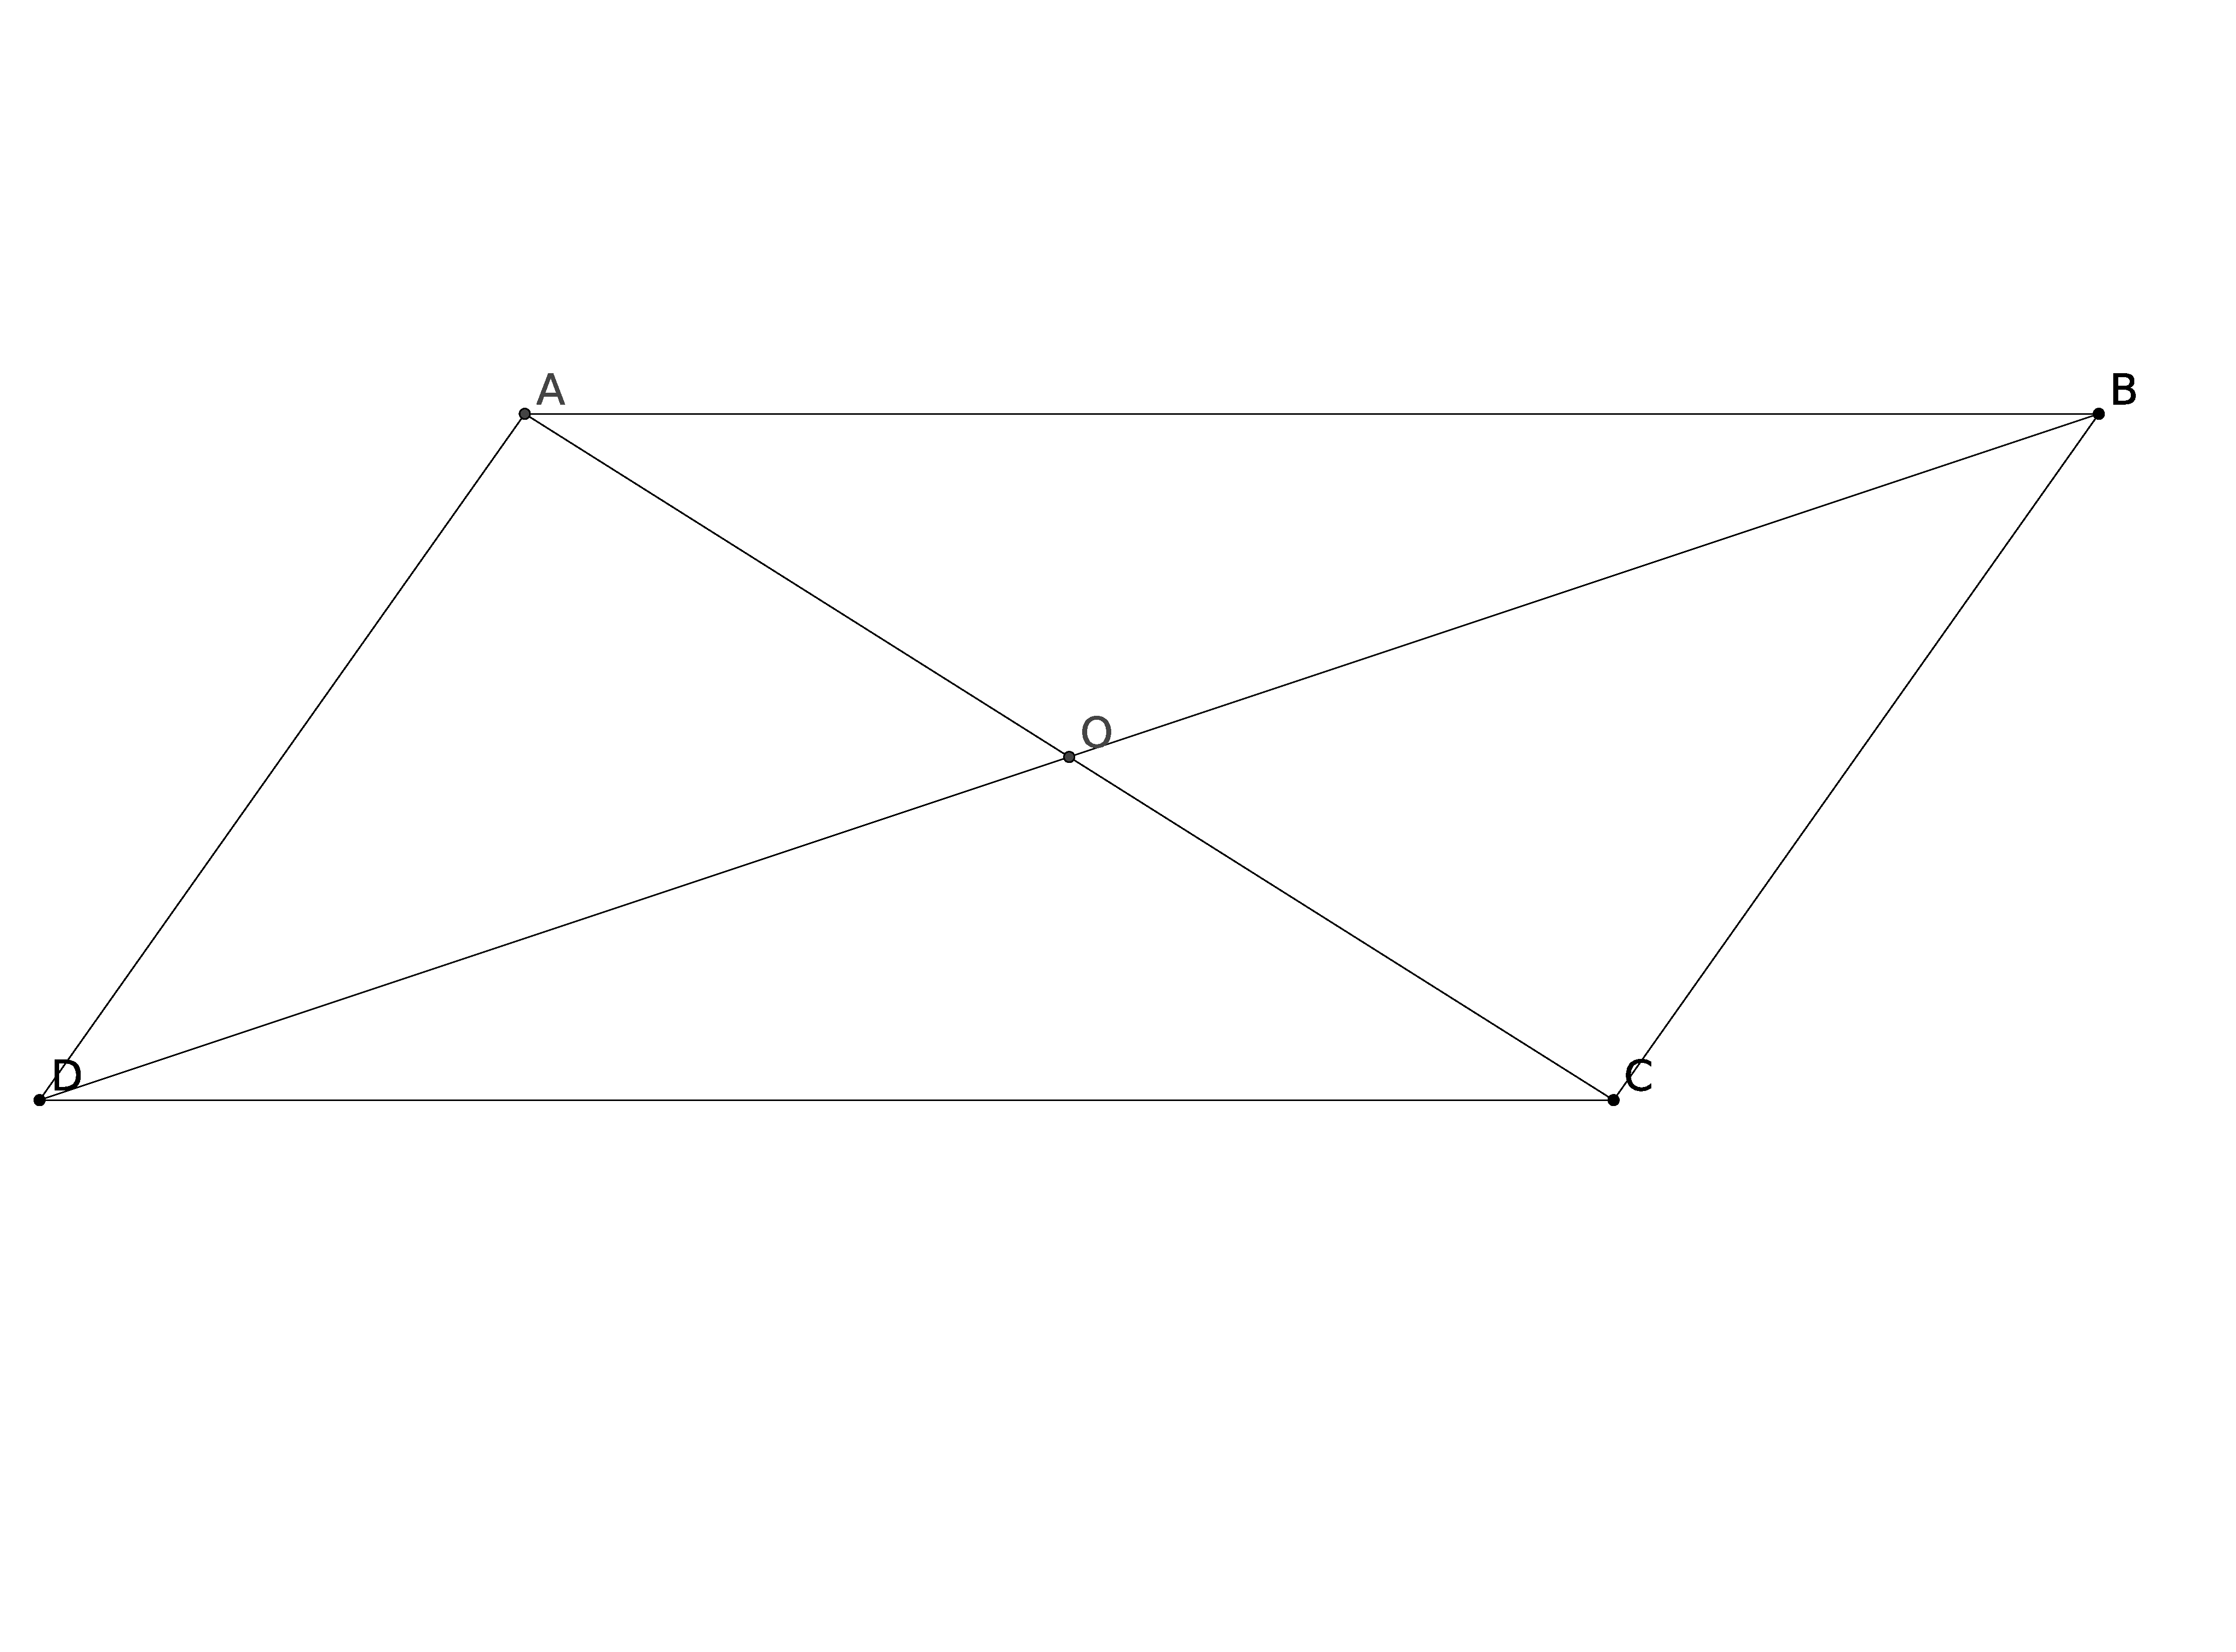
\includegraphics[scale=0.2]{parallelogram1.eps}
    \end{figure}
    
    
\begin{hyp}
$ABCD$ est un parallélogramme, donc $AB \parallel DC$ et $AD \parallel BC$.
\end{hyp}

\begin{concl}
$AO \equiv OC$, $DO \equiv OB$
\end{concl}
Puisque la définition du parallélogramme n'implique pas que les côtés opposés d'une telle figure sont isométriques, nous commençons par démontrer cela. \\
Ainsi, nous considérons les deux triangles $\triangle ABC$ et $\triangle ACD$ et nous remarquons qu'il sont isométriques grâce au théorème de la transversale (théorème \ref{th:transversale}).

\begin{figure}[H]
        \centering
        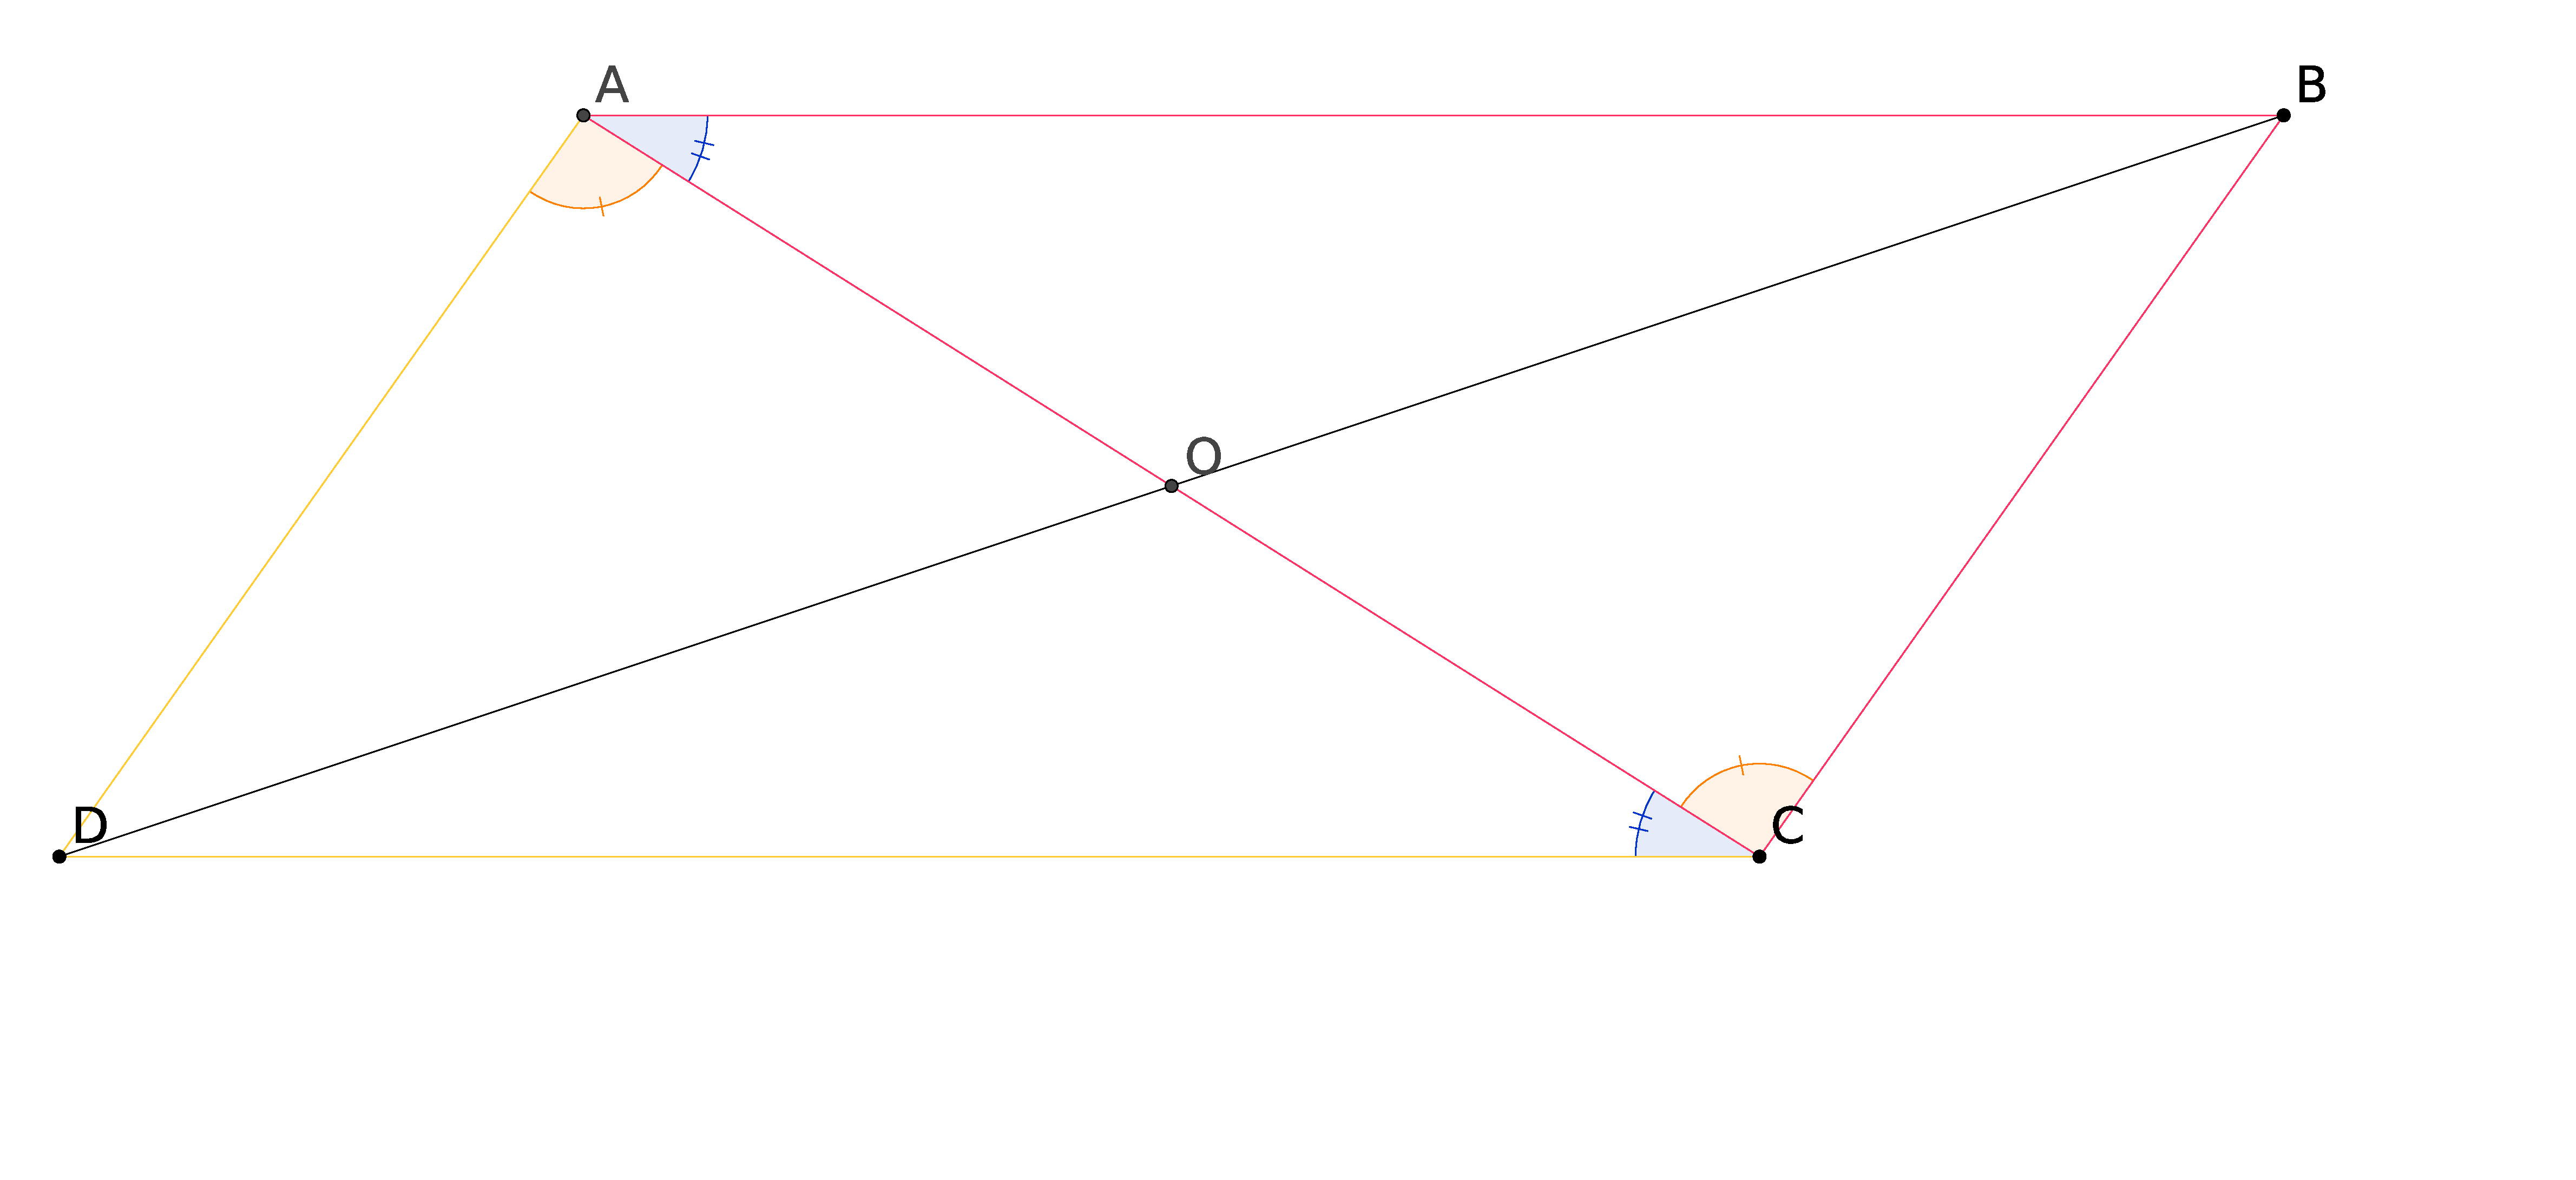
\includegraphics[scale=0.2]{parallelogram2.eps}
    \end{figure}

En effet, ces triangles respectent le deuxième cas d'isométrie des triangles, car $\angle DAC \equiv \angle ACB$, $\angle DCA \equiv \angle CAB$ et les deux triangles partagent $AC$. Nous avons donc $AB \equiv DC$ et $AD \equiv BC$.\\

A présent, grâce à l'isométrie de deux angle opposés par le sommet, on observe que que les paires d'angles $\angle AOB$/$\angle DOC$ et $\angle AOD$/$\angle COB$ sont isométriques. 

\begin{figure}[H]
        \centering
        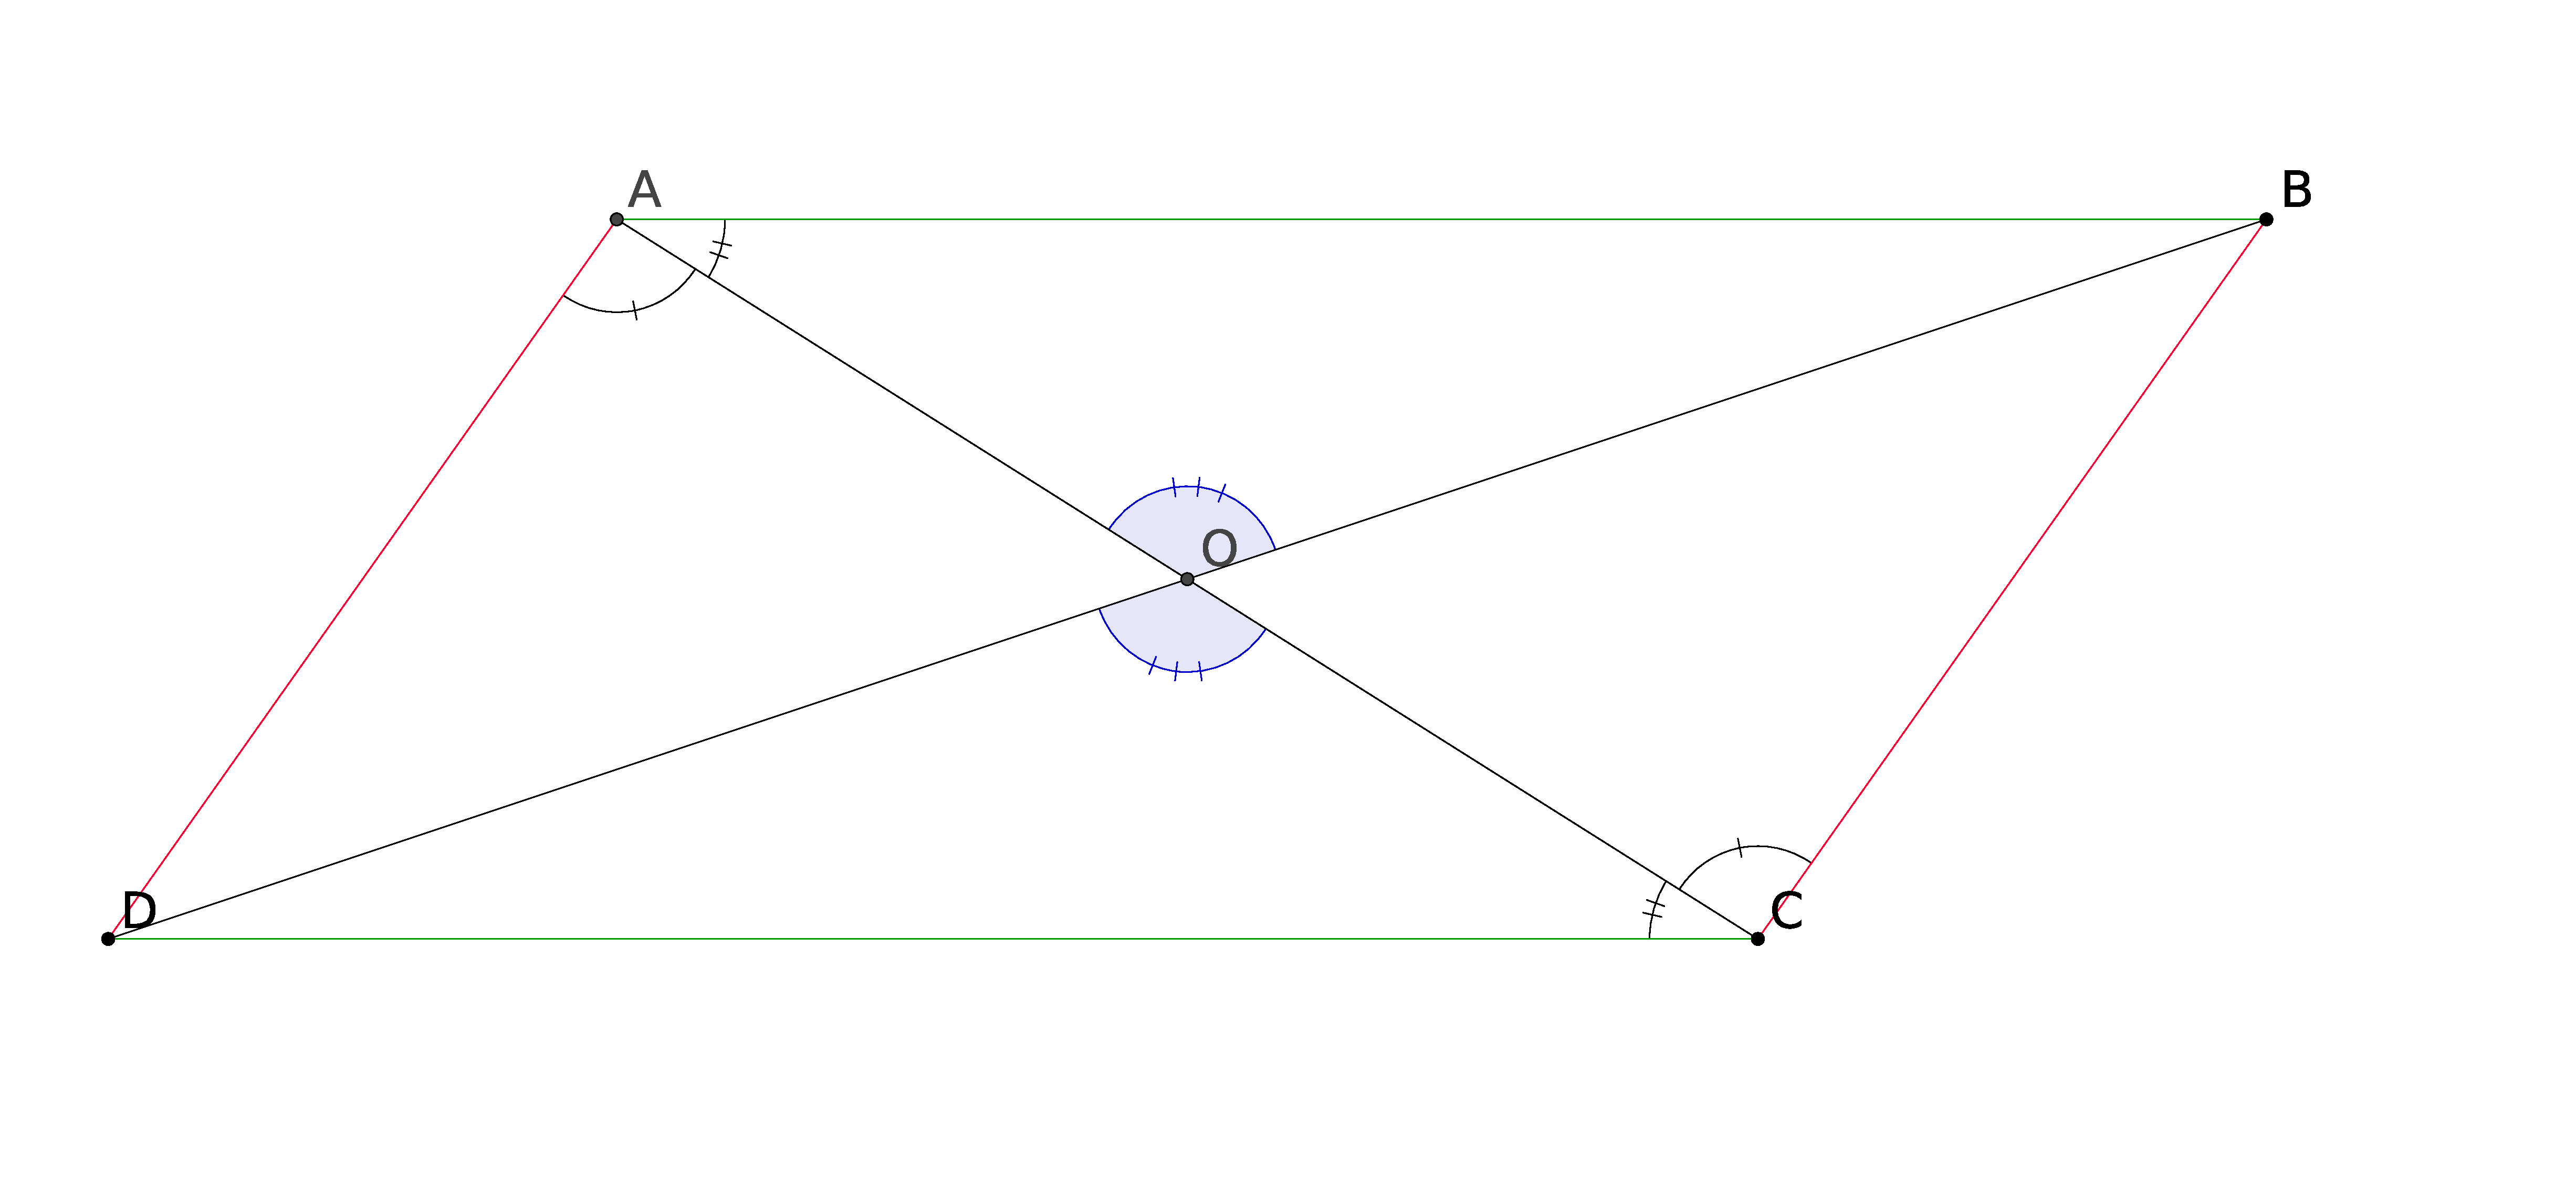
\includegraphics[scale=0.2]{parallelogram3.eps}
    \end{figure}

Par conséquent, grâce au corollaire du deuxième cas d'isométrie des triangles, les paires de triangles $\triangle AOD$/$\triangle COB$ et $\triangle AOD$/$\triangle COB$ sont isométriques. Ainsi, $AO \equiv OC$ et $DO \equiv OB$. Nous avons donc démontré que les diagonales d'un parallélogramme se coupent en leur milieu.
\end{proof}

\end{document}

\documentclass[a4paper,12pt]{article}

\input{packages}

\begin{document}
\pagebreak
\subsection{Théorème des médiatrices}

\begin{theorem}
La médiatrice d'un segment est le lieu géométrique des points équidistants à ses extrémités.
\end{theorem}

%insert figure

Pour démontrer ce théorème, nous devons prouver les deux affirmations suivantes:
\begin{enumerate}
    \item Tout point se situant sur la médiatrice d'un segment se situe à la même distance de ses deux extrémités.
    \item Tout point se trouvant à égale distance de deux autres points se situe sur la médiatrice du segment défini par ces derniers.\\
\end{enumerate}


\begin{enumerate}
    \item \begin{proof}
    Nous considérons le segment $AB$, ayant $m$ comme médiatrice. $M$ est le point à l'intersection de $m$ et du segment $AB$.
    
    \begin{hyp}
    $P \in m$ 
    \end{hyp}
    \begin{concl}
    $AP \equiv BP$
    \end{concl}
     
    Grâce au premier cas d'isométrie des triangles, nous observons que les triangles $\triangle AMP$ et $\triangle BMP$ sont isométriques car ils ont un côté en commun ($MP$) et que $AM$ et $MB$ sont isométriques. Par conséquent, $AP \equiv BP$.
     \end{proof}
     
    \item \begin{proof}
         Nous considérons un point $P$ à égale distance de deux autres point, $A$ et $B$. 
        
        \begin{hyp}
        $AP \equiv BP$
        \end{hyp}
        \begin{concl}
        $P \in m$
        \end{concl}
        Nous traçons le segment $MP$ et observons que c'est la médiane du triangle formé par les points $A$, $P$ et $B$, car il part        de l'un des sommet du triangle et partage le côté opposé en deux parties égales. Ainsi, nous observons que les angles $\angle      APM$ et $\angle MPB$ sont isométriques.  Par conséquent, les triangles $\triangle AMP$ et $\triangle BMP$ sont isométriques      car ils possèdent un angle isométrique ($\angle APM \equiv \angle MPB$) compris entre deux côtés isométriques ($AP \equiv      BP$, par hypothèse et $MP$ en commun). Finalement, le segment $MP$ et la médiatrice de $AB$ sont confondus et $P \in m$.\\
        \end{proof}
\end{enumerate}

\end{document}
 
\documentclass[a4paper,12pt]{article}

\input{packages}

\begin{document}

\begin{corollary} \label{cor:mediatrices}
Les médiatrices d'un triangle se croisent en un point unique, le centre du cercle circonscrit du triangle $ABC$.
\end{corollary}
\begin{proof}
Nous considérons un triangle quelconque $ABC$. Nous nommons $I$ l'intersection des médiatrices des côtés $AC$ ($M_{AC}$) et $BC$ ($M_{BC}$).

\begin{hyp}
$I \in M_{AC}$ et $I \in M_{BC}$
\end{hyp}
\begin{concl}
$I \in M_{AB}$ (la médiatrice du côté $AB$) 
\end{concl}

En considérant l'hypothèse et la définition de la médiatrice (définition \ref{def:mediatrice}), nous savons que $IA \equiv IC$ et que $IB \equiv IC$. Par conséquent, $IA \equiv IB$. Puisque $I$ est à une distance équivalente de $A$ et de $B$, $I \in M_{AB}$.\\
De plus, puisque $I$ est le lieu des points équidistants à $A$, $B$ et $C$, c'est aussi le cercle du cercle circonscrit de $\triangle ABC$.
\end{proof}

\end{document}

\documentclass[a4paper,12pt]{article}

\input{packages}

\begin{document}

\subsection{Théorème de l'intersection des médianes}
\begin{theorem}
La médiatrice d'un segment est le lieu géométrique des points équidistants à ses extrémités.
\end{theorem}

\end{document}

\documentclass[a4paper,12pt]{article}

\input{packages}

\begin{document}

\subsection{Théorème de l'intersection des hauteurs}
\begin{theorem}
Les hauteurs d'un triangle concourent en un seul point nommé orthocentre.
\end{theorem}

\begin{proof}
Nous considérons le triangle quelconque $ABC$, ayant $h_A$ comme hauteur passant $A$.
\begin{hyp}
$\triangle ABC$ est quelconque
\end{hyp}
\begin{concl}
les hauteurs de $\triangle ABC$ concourent en un seul point
\end{concl}
Nous construisons les points $D$, $E$ et $F$ ainsi que:
\begin{itemize}
    \item $DE \parallel CB$
    \item $EF \parallel CA$
    \item $DF \parallel AB$
\end{itemize}
Dès lors, nous obtenons par construction deux parallélogrammes $AEBC$ et $DABC$ (ils ont deux paires de côtés parallèles). Cela implique que $AE \equiv CB$ et $DA \equiv CB$ (théorème \ref{th:parallelogramme}) et donc $AE \equiv DA$. Ainsi, $h$ est la médiatrice du segment $DE$. Les hauteurs du triangle $ABC$ sont donc les médiatrices du triangle $DEF$. Cela signifie que les hauteurs d'un triangle concourent en un point, car elles sont confondues avec les médiatrices d'un triangle augmenté, or nous avons démontré que les médiatrices d'un triangle s'intersectent en un seul point (corollaire \ref{cor:mediatrices}).
\end{proof}

\end{document}

\input{theorems/semblables/semblables}
\documentclass[a4paper,12pt]{article}

\input{packages}

\begin{document}

\subsubsection{Théorème 1}
\begin{theorem}
Deux triangles dont les côtés sont respectivement parallèles ont des angles respectivement isométriques.
\end{theorem}

\begin{proof}
Nous considérons deux triangles quelconques $\triangle ABC$ et $\triangle A'B'C'$.



\begin{figure}[H]
        \centering
        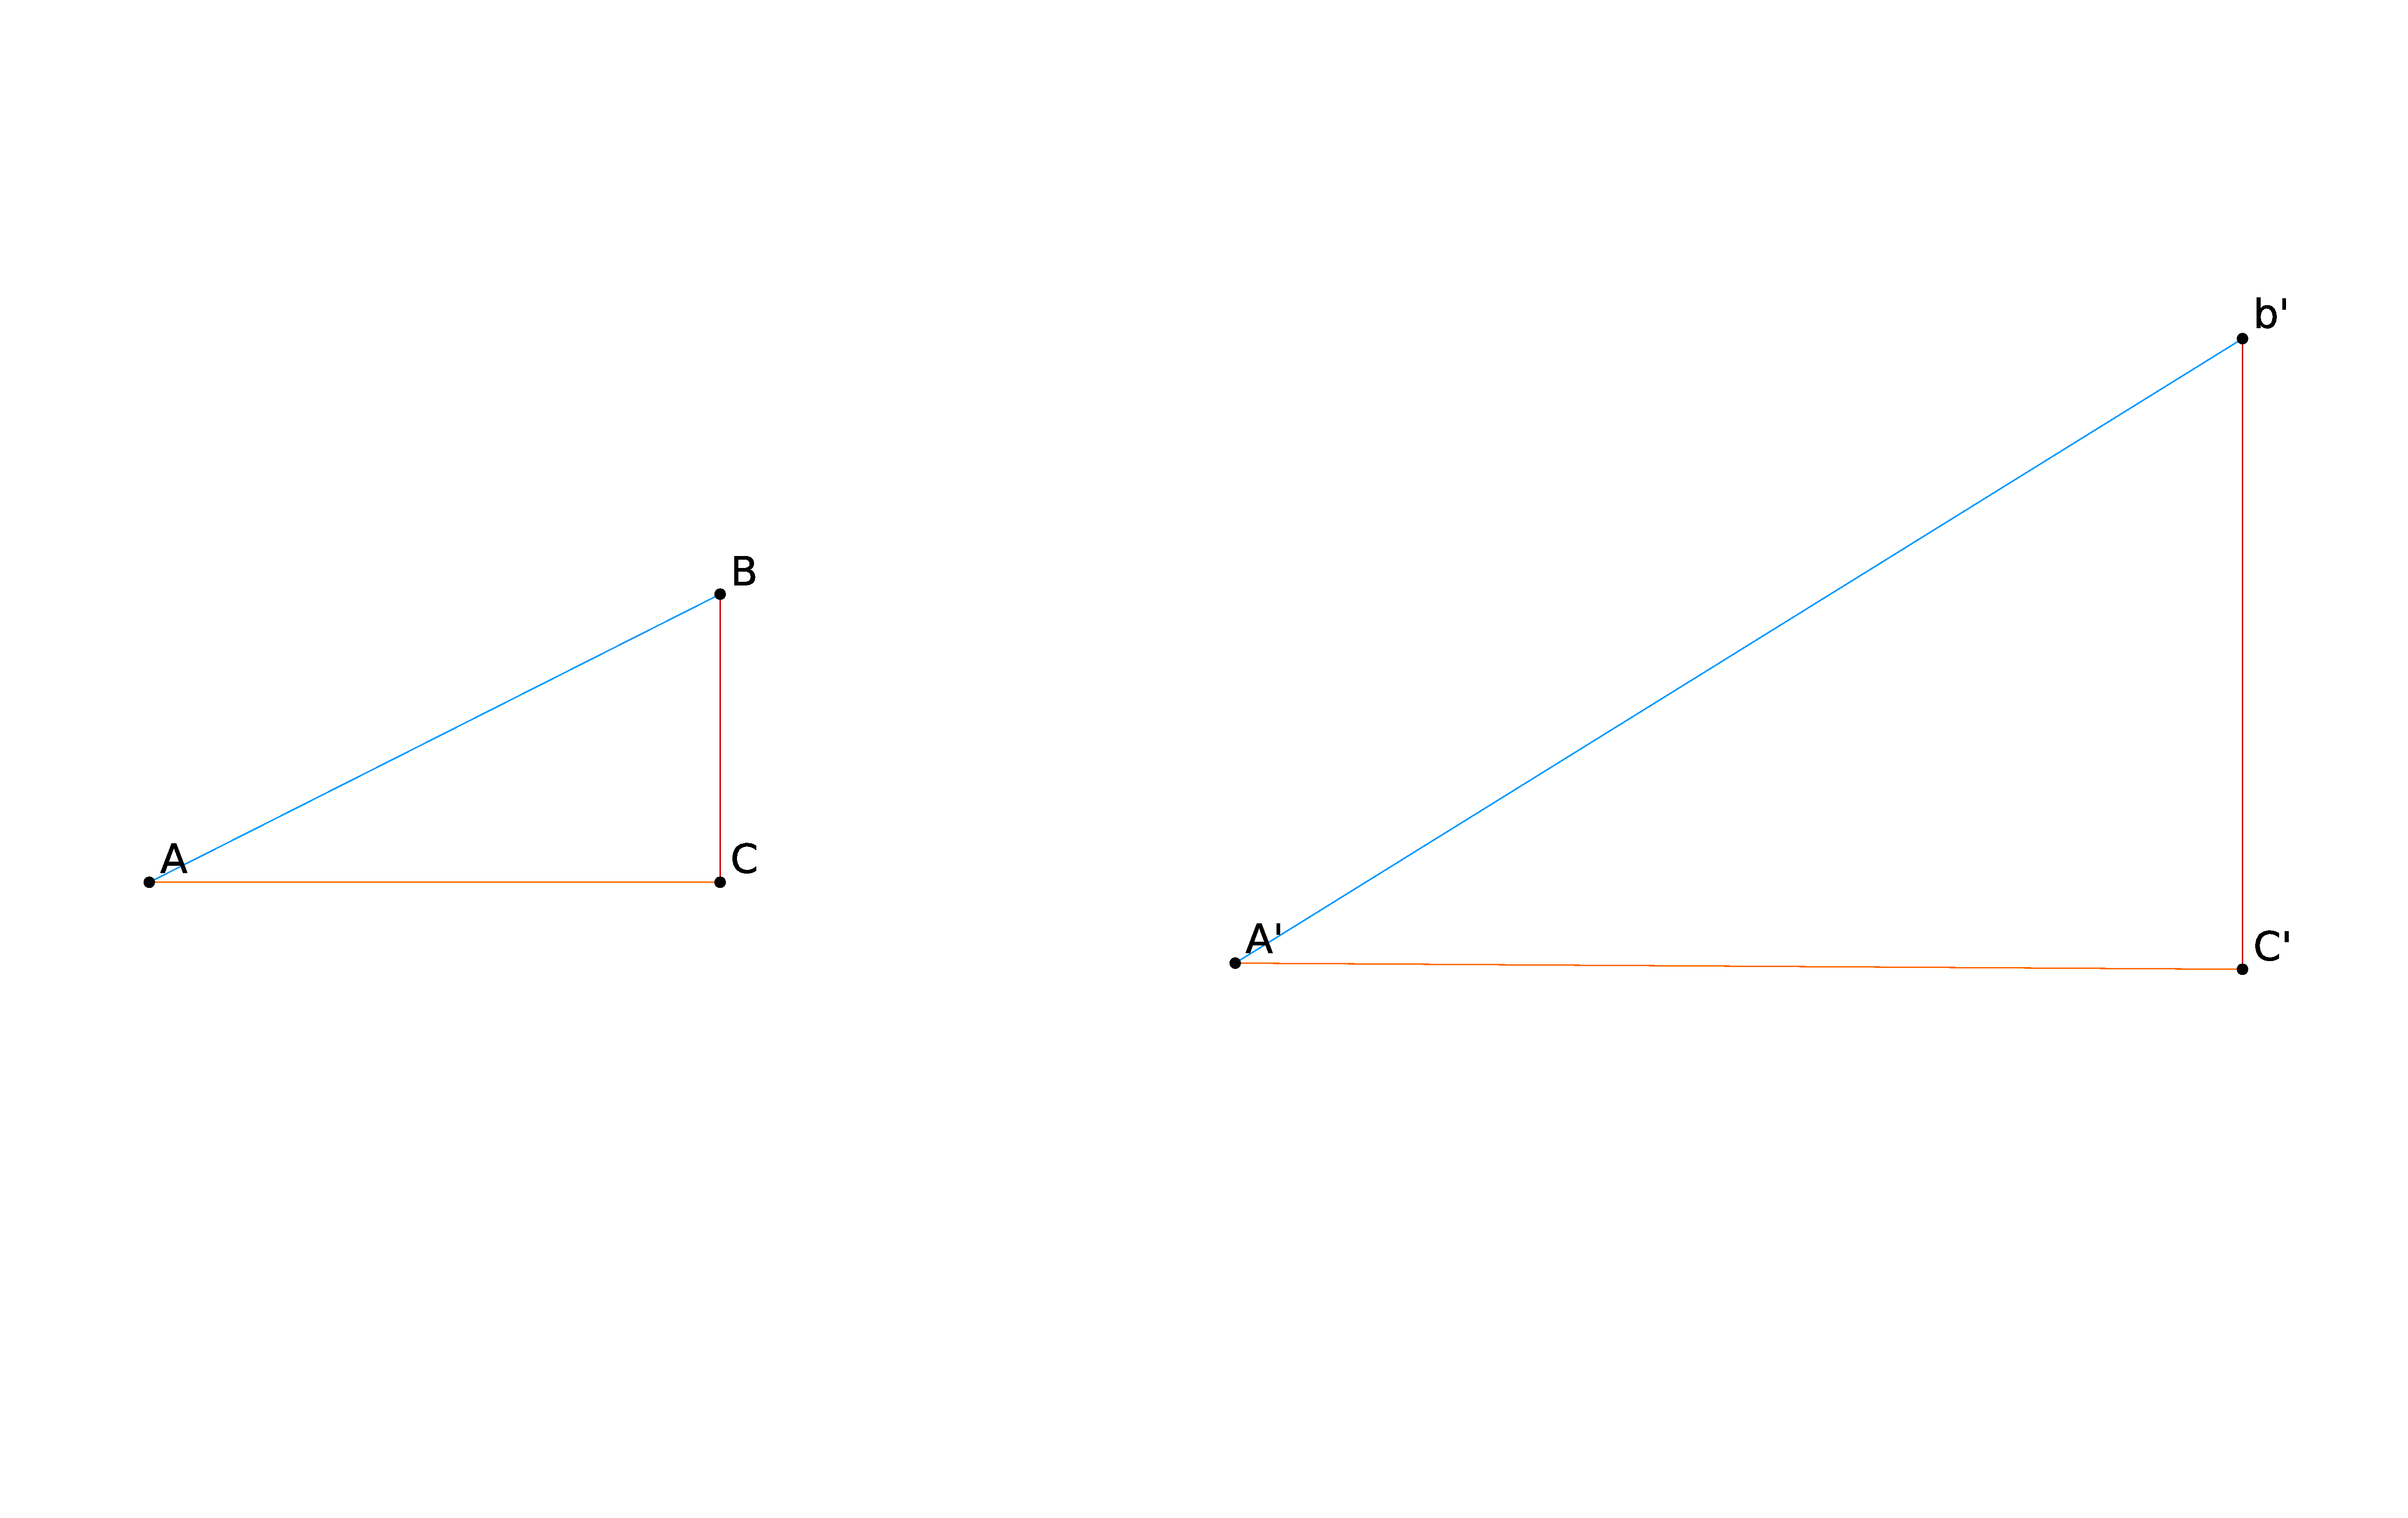
\includegraphics[scale=0.2]{semblable1.1.eps}
    \end{figure}

\begin{hyp}
$a \parallel a'$, $b \parallel b'$ et $c \parallel c'$
\end{hyp}
\begin{concl}
$\alpha \equiv \alpha'$, $\beta \equiv \beta'$ et $\gamma \equiv \gamma'$
\end{concl}

Nous prolongeons $a$, $a'$ et $c'$. 

\begin{figure}[H]
        \centering
        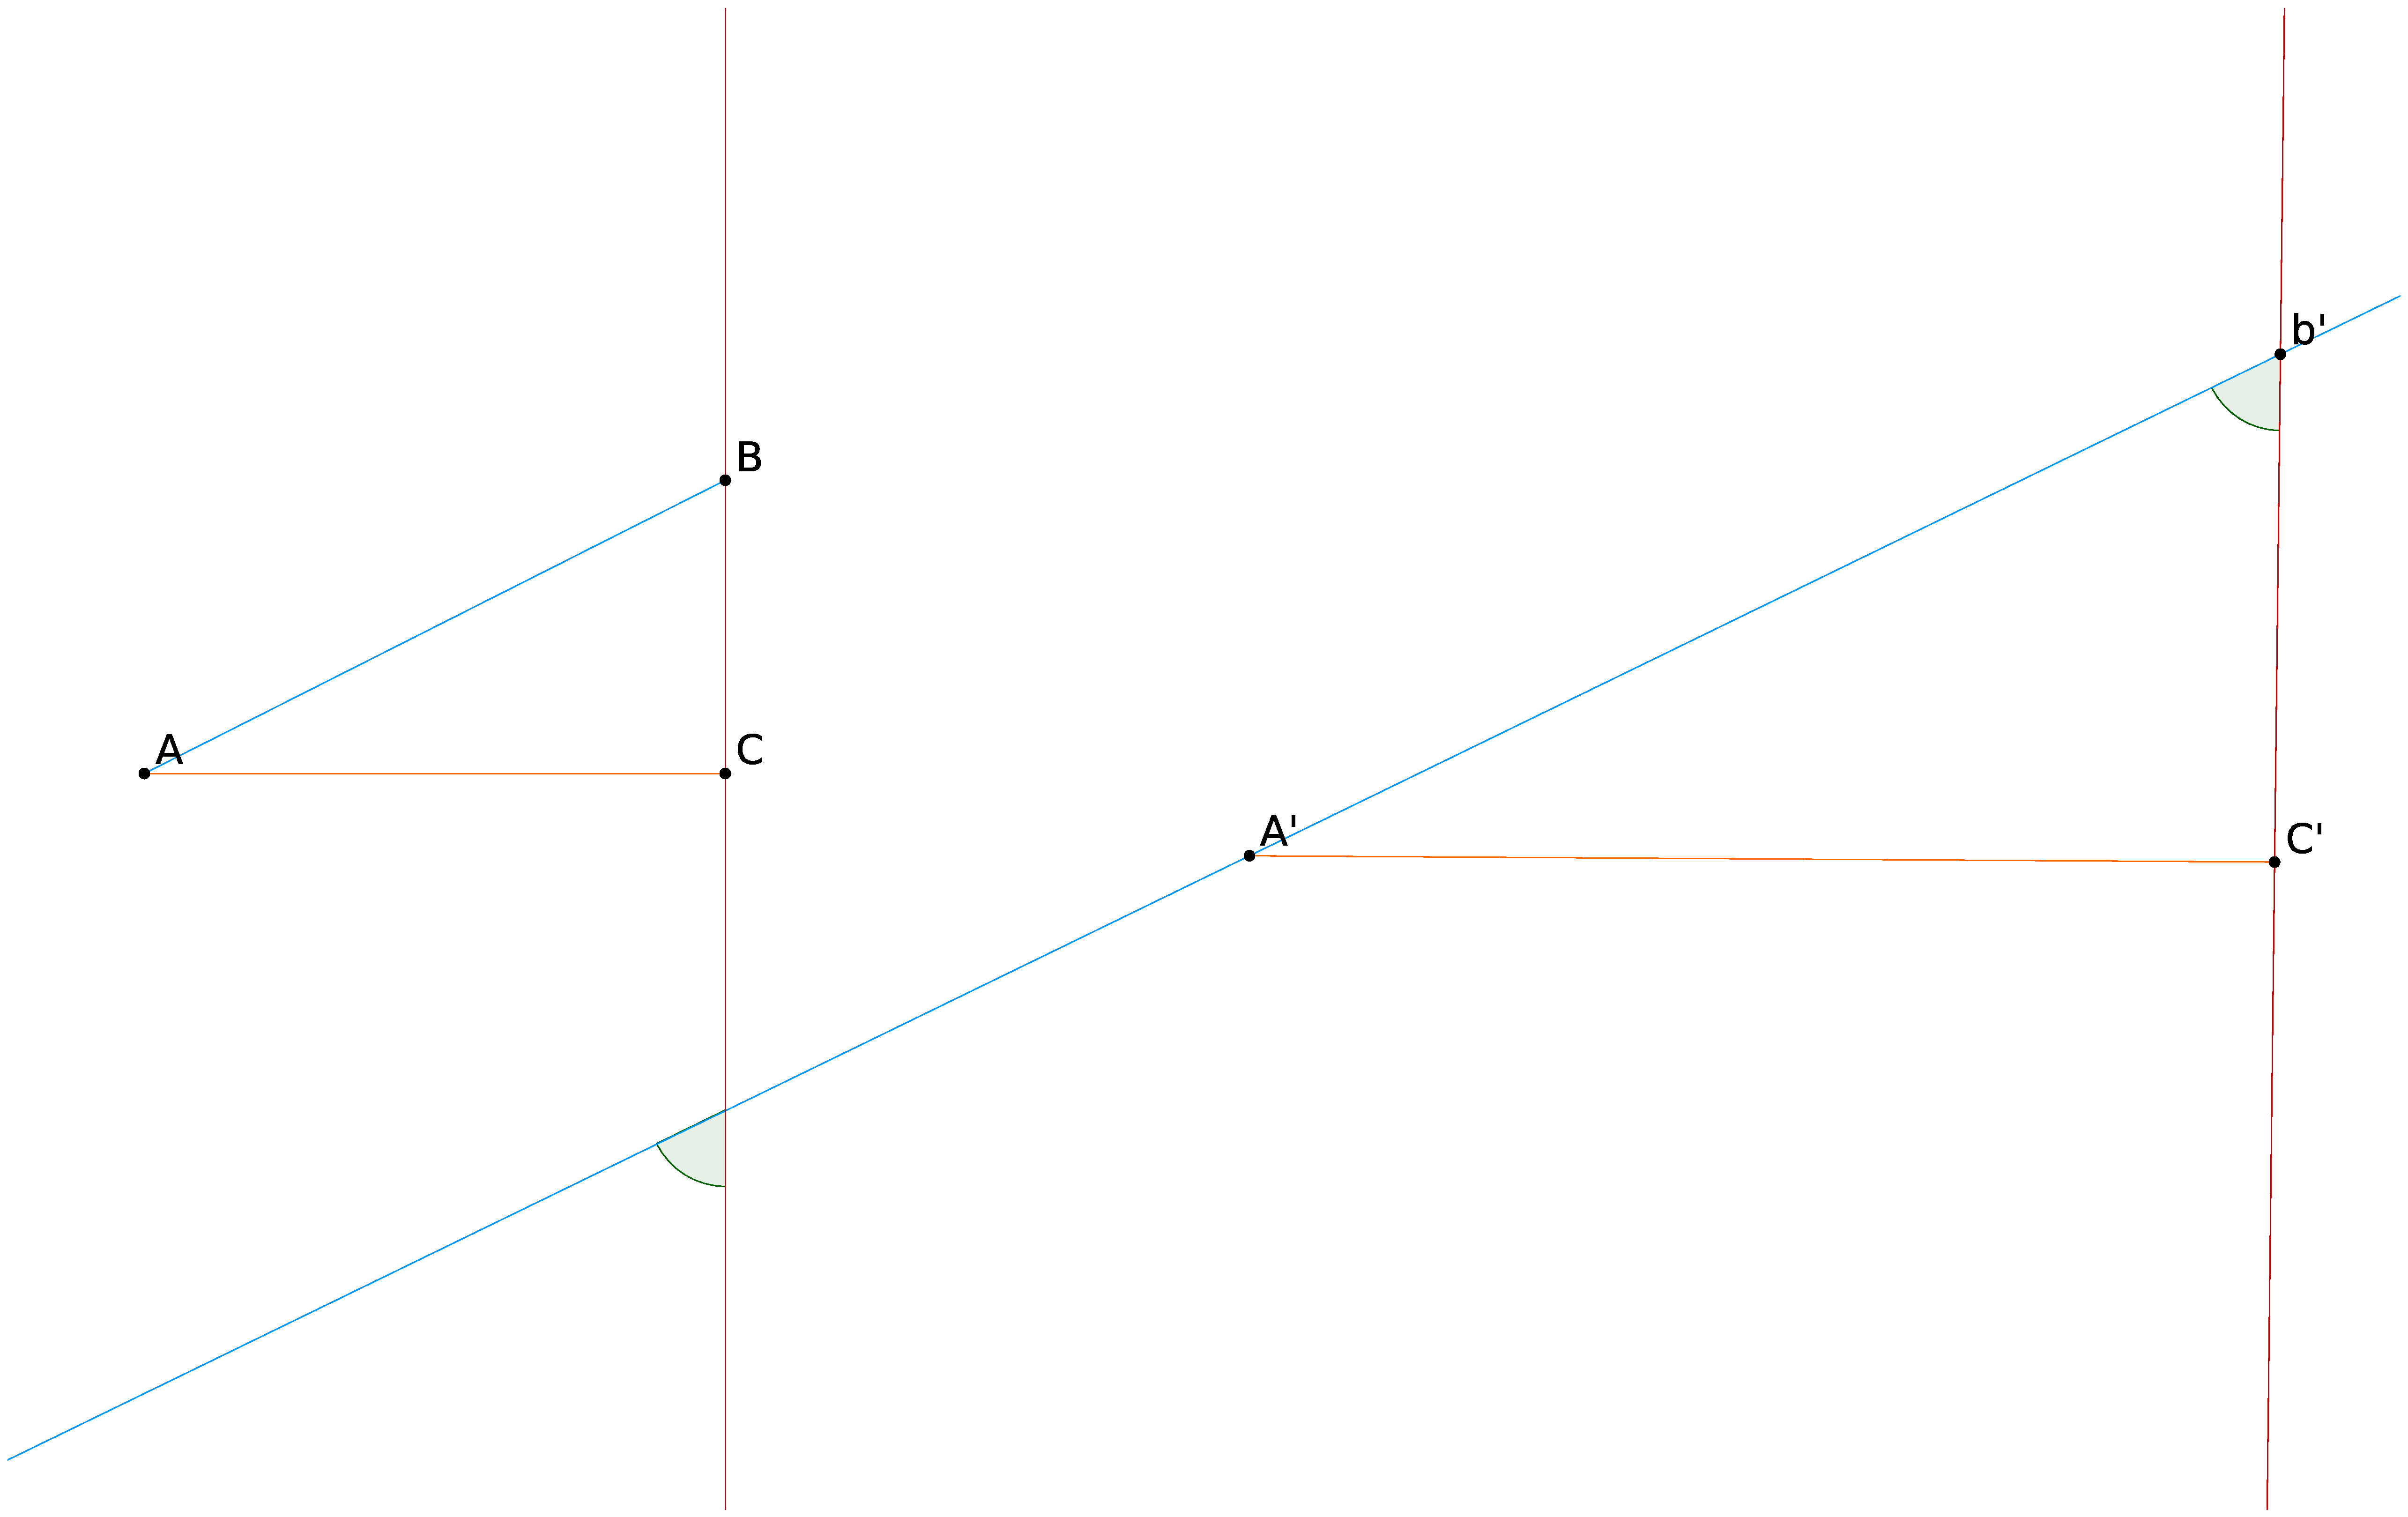
\includegraphics[scale=0.2]{semblable1.2.eps}
    \end{figure}

Grâce au théorème de la transversale, nous observons que $\beta' \equiv \theta$, où theta est l'angle correspondant de beta.\\
Nous prolongeons $c$, $c'$ et $a$ et grâce au même théorème qu'auparavant, nous savons que $\beta \equiv \theta$.
Ainsi, $\beta \equiv \beta' \equiv \theta$.\\
Il suffit de répéter cette démonstration pour les deux autres angles des triangles afin d'obtenir $\alpha \equiv \alpha'$, $\beta \equiv \beta'$ et $\gamma \equiv \gamma'$.

\begin{figure}[H]
        \centering
        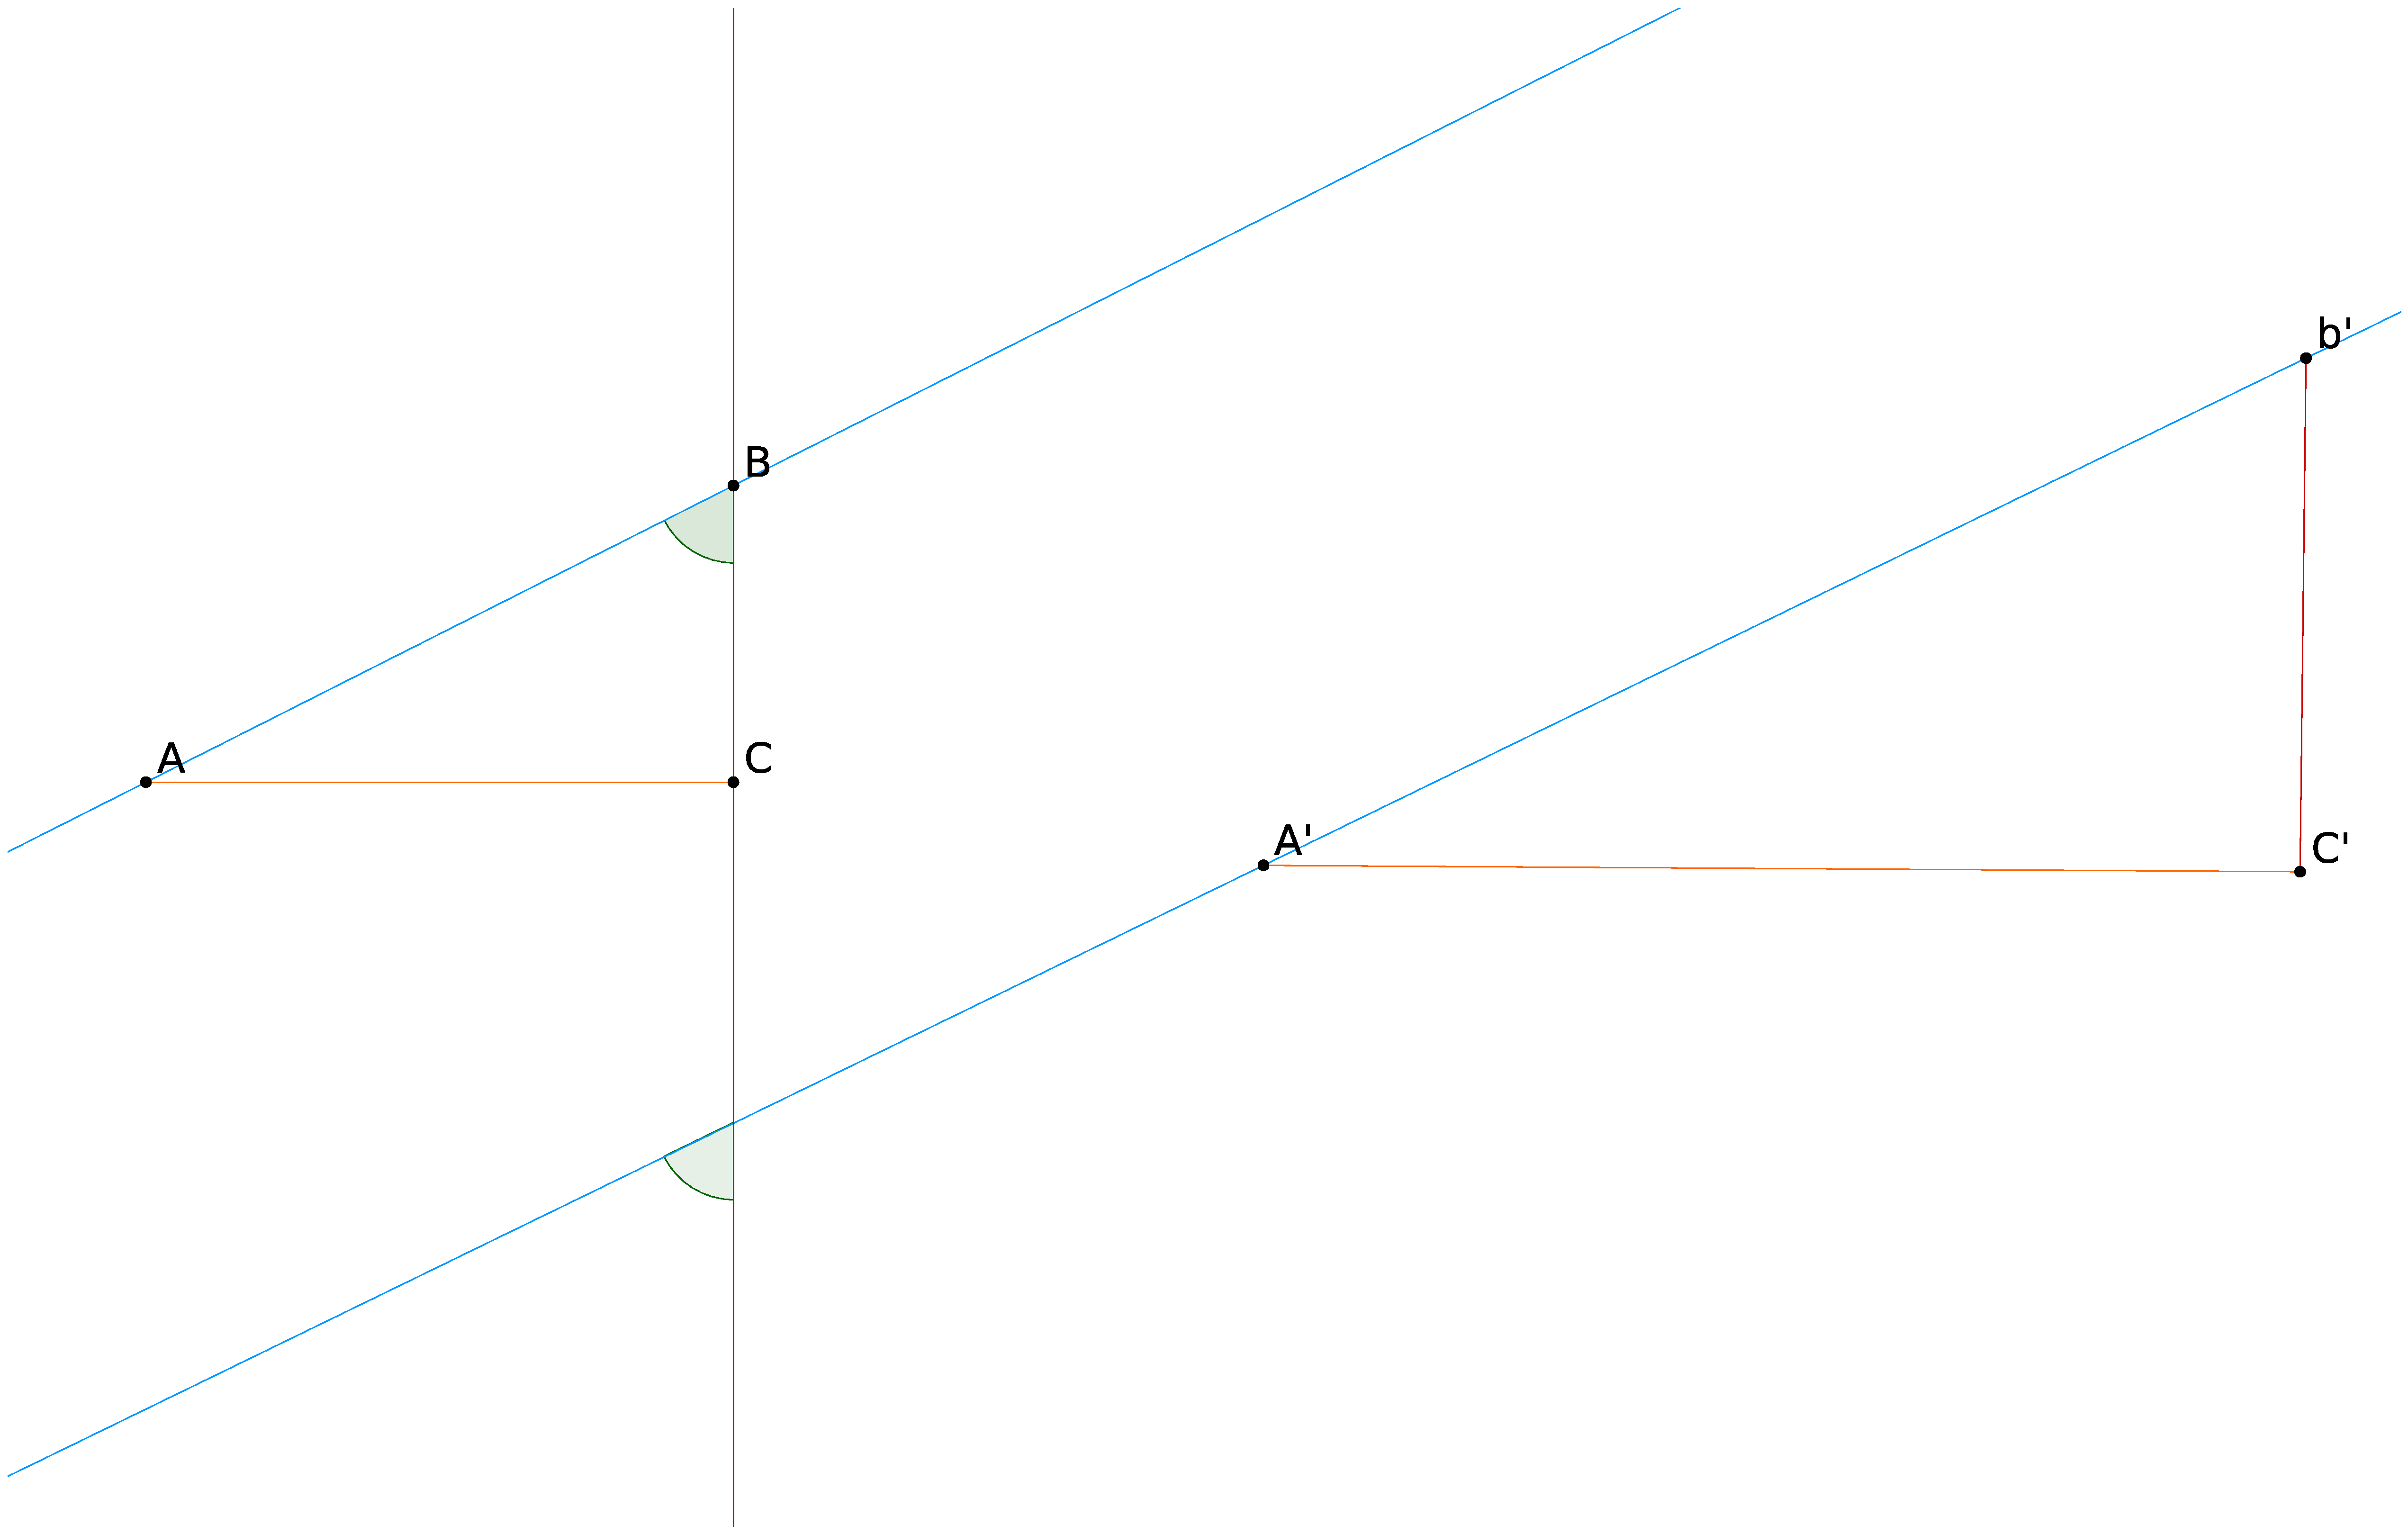
\includegraphics[scale=0.2]{semblable1.3.eps}
    \end{figure}

\end{proof}

\end{document}
\documentclass[a4paper,12pt]{article}

\input{packages}

\begin{document}

\pagebreak
\subsubsection{Théorème 2}
\begin{theorem}\label{semblableTh2}
Si deux paires de parallèles découpent sur une sécante deux segment isométriques, elles le font sur toute autre sécante.
\end{theorem}

\begin{proof}
Nous considérons la droite $m$ qui a $m'$ comme sécante et deux paires de parallèles ($a$, $b$, $c$ et $d$) qui interceptent m et m' en huits point (respectivement $A$, $B$, $C$, $D$, $A'$, $B'$, $C'$, et $B'$). Nous construisons les parallèles de sorte à ce que $AB \equiv CD$.

\begin{figure}[H]
        \centering
        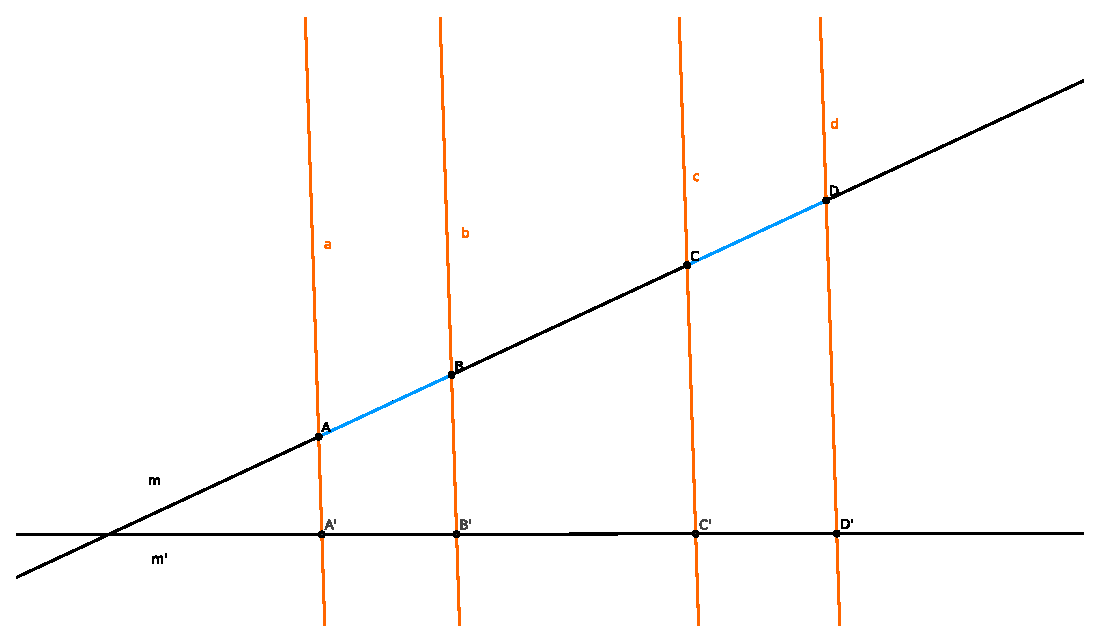
\includegraphics[scale=0.9]{semblable2-1.eps}
    \end{figure}

\begin{hyp}
\begin{itemize}
    \item $m \cap m'$
    \item a, b c et d sont parallèles
    \item $AB \equiv CD$
\end{itemize}
\end{hyp}
\begin{concl}
$A'B' \equiv C'D'$
\end{concl}
Nous construisons deux droites $e$ et $f$ qui passent respectivement par $A$ et $D$ et sont parallèles à $m'$.\\
Nous nommons $E = e \cap b$ et $F = f \cap c$.\\
Grâce au théorème de la transversale, nous savons que $\angle ABE \equiv \angle FCD$ et $\angle BAE \equiv \angle FDC$. Nous pouvons en déduire que $\triangle ABE$ et $\triangle FCD$ sont isométriques ($2^{me}$ cas d'isométrie des triangles).\\
\begin{figure}[H]
        \centering
        \includegraphics[scale=0.9]{semblable2-2.eps}
    \end{figure}

Cela signifie que $AE \equiv FD$, or par construction, nous savons que  les quadrilatères $AEA'B'$ et $FDC'D'$ sont des parallèlogrammes (définition des parallèlogrammes) et que $A'B' \equiv C'D'$.
\begin{figure}[H]
        \centering
        \includegraphics[scale=0.9]{semblable2-3.eps}
    \end{figure}
    
\end{proof}

\end{document}
\documentclass[a4paper,12pt]{article}

\input{packages}

\begin{document}

\pagebreak
\subsubsection{Théorème 3 (théorème de Thalès)}
\begin{theorem}
Deux paires de parallèles qui découpent sur une droite deux segments proportionnels découpent des segments de mèeme proportion sur toute sécante de la première droite.
\end{theorem}

\begin{proof}
Nous considérons le triangle quelconque $ABC$ 
\begin{hyp}

\begin{itemize}
    \item $m$ et $m'$ deux droites, $m \cap m'$
    \item $a$, $b$ $c$ et $d$ sont quatre droites parallèles qui interceptent $m$ et $m'$ respectivement en $A$, $B$, $C$ et $D$ et $A'$, $B'$, $C'$ et $D'$.
\end{itemize}

\end{hyp}

\begin{concl}
$\frac{AB}{CD} = \frac{A'B'}{C'D'}$
\end{concl}
\begin{figure}[H]
        \centering
        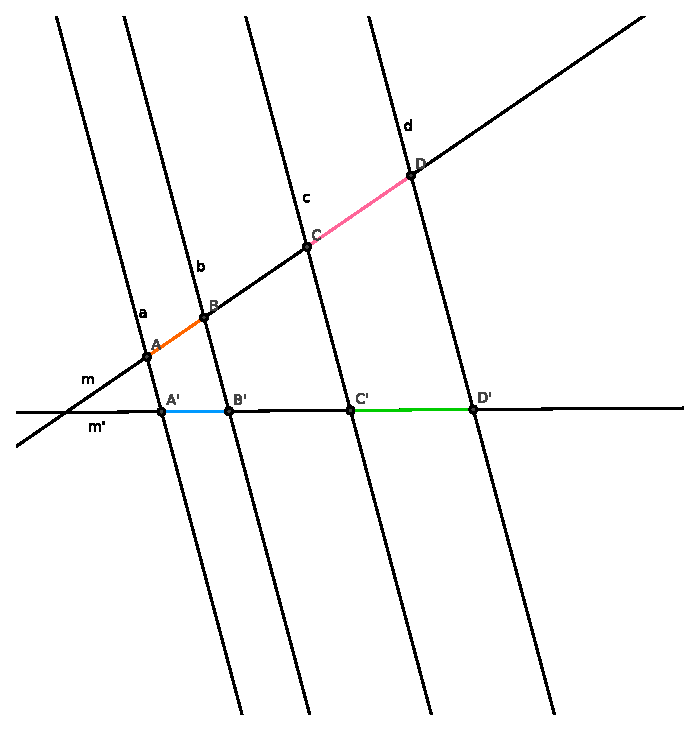
\includegraphics[scale=1.2]{thales1.eps}
    \end{figure}

\begin{remark}
Notre démonstration ne peut être utilisée qu'avec des nombres rationnels. En effet, celle pour les nombres réels est bien plus complexe et nous ne l'aborderons pas.
\end{remark}

Afin de démontrer ce théorème pour les nombres rationnels, nous exprimons le ratio $\frac{AB}{CD}$ sous une forme rationnelle, c'est-à-dire sous forme $\frac{p}{q}$. Nous réalisons la démonstration avec $\frac{AB}{CD} = \frac{3}{5}$, une valeur numérique, afin de faciliter la compréhension de la démonstration.\\

Nous commençons par diviser $AB$ en trois parties isométriques et $CD$ en cinq. Nous nommons respectivement $EF$ et $GH$ un des segments ainsi formés.
Ainsi nous obtenons que $AB = 3EF$ et $CD = 5EF$. Donc $\frac{3EF}{5GH} = \frac{AB}{CD} = \frac{3}{5}$ et l'on observe que $EF \equiv GH$.\\

\begin{figure}[H]
        \centering
        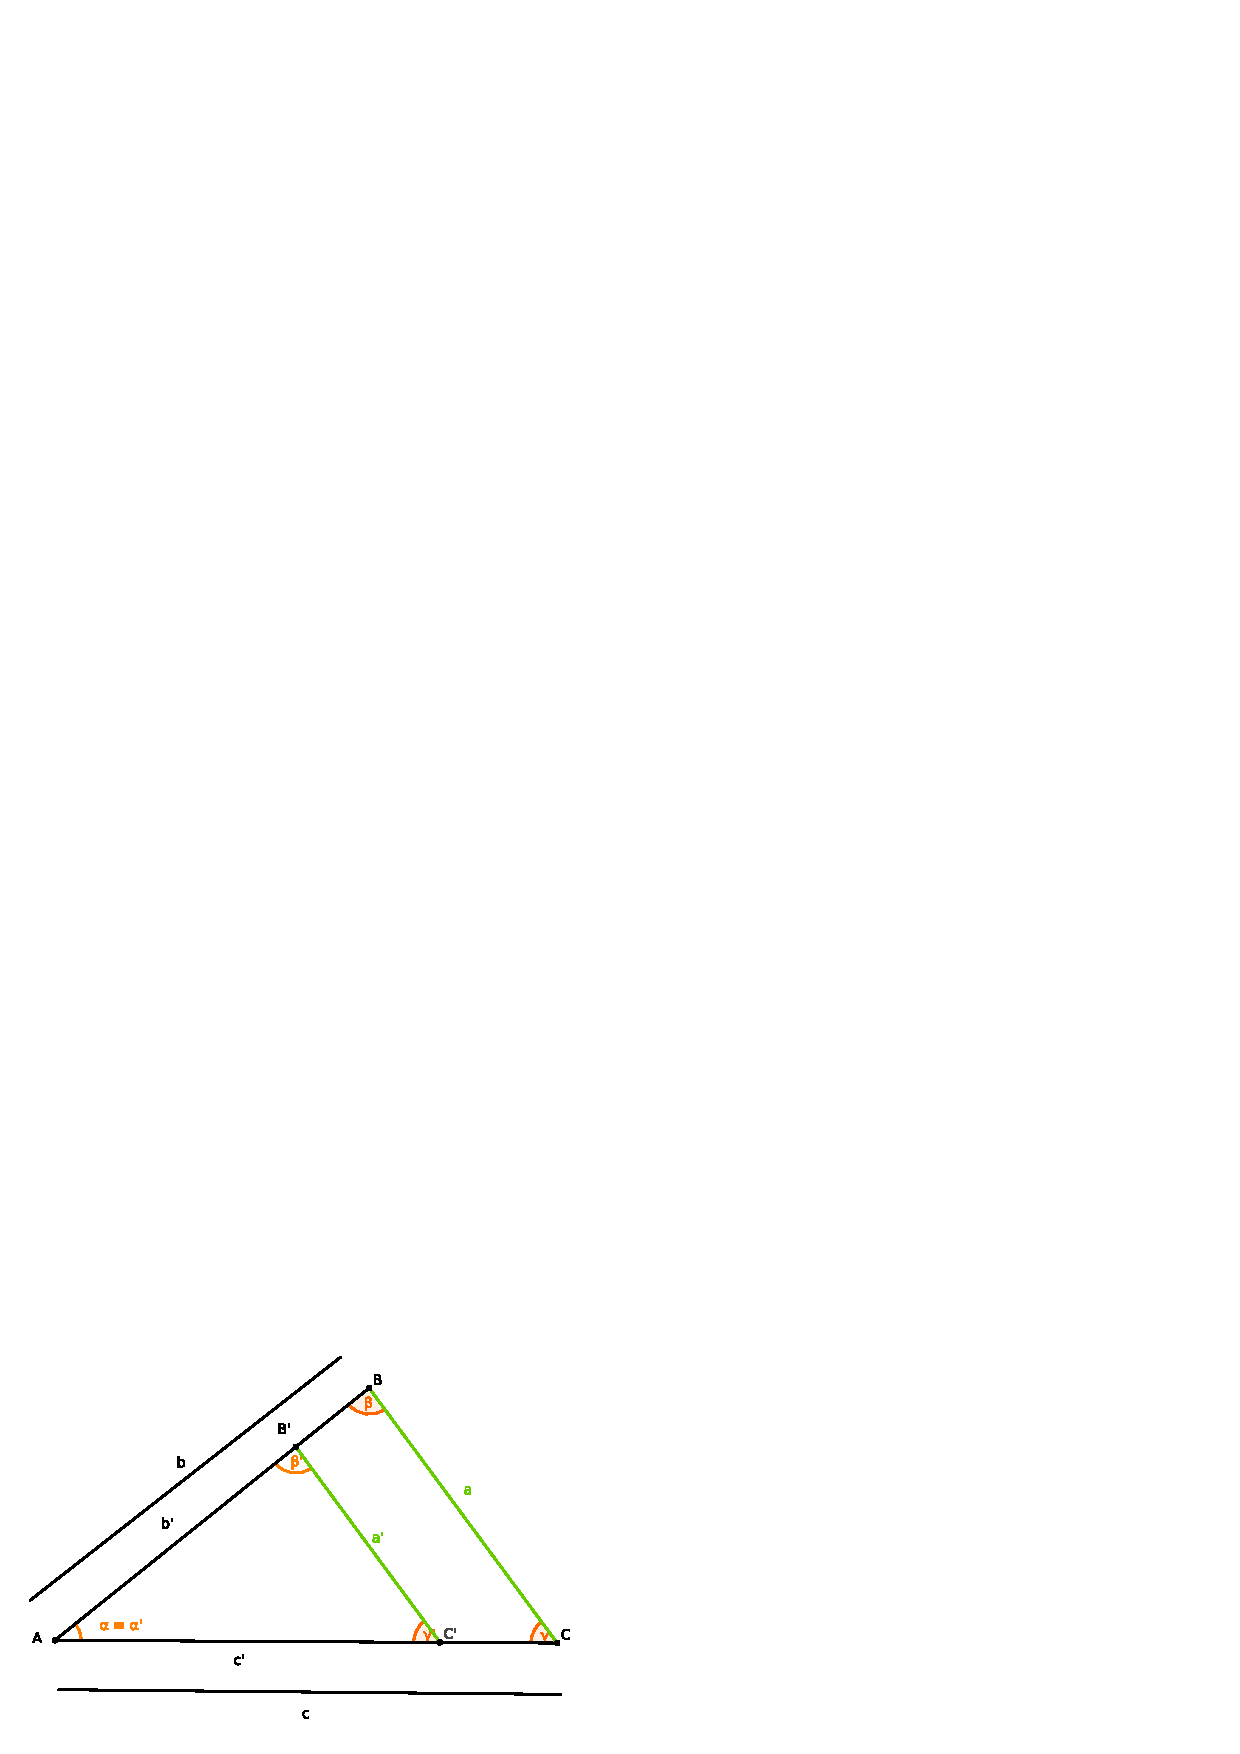
\includegraphics[scale=1.1]{thales2.png}
    \end{figure}

 Dès lors, si l'on trace des droites parallèles aux premières et passant par les points $E$, $F$, $G$ et $H$, l'on sait que les segments qu'elles découpent sur $m'$ sont isométriques (grâce au théorème précédent, théorème \ref{semblableTh2}). Nommons deux de ces segments $E'F'$ et $G'H'$, alors $\frac{AB}{CD} = \frac{3}{5} = \frac{3E'F'}{5G'H'} = \frac{A'B'}{C'D'}$.
Ainsi, si on généralise cette démonstration à $\frac{A'B'}{C'D'} = \frac{p}{q}$, on démontre le théorème de Thalès pour tous les nombre rationnels.
\end{proof}




\pagebreak
\begin{remark}
Thalès vécu au septième et sixième siècle avant J.C. dans la ville de Milet, en Grèce. Marchand de profession, il est aussi philosophe et l'un des précurseurs de la pensée scientifique moderne. En effet, au lieu de reposer l'explication de phénomènes inexpliqués sur la mythologie, il privilégia l'observation et son expérience personnelle. Ce procédé lui permit de faire de nombreuses découvertes et inventions d'une grande importance, notamment en astronomie, physique et mathématiques.\\
\begin{figure}[H]
    \centering
    \includegraphics[scale = 0.2]{theorems/semblables/thales/thales.jpg}
    
    \caption{Portrait de Thalès de Milet}
    \label{fig:thales}
\end{figure}

\pagebreak
On lui accorde, entre autre, la découverte d'un moyen de mesurer la hauteur des pyramides d'Egypte. Il observa qu'il existe chaque jour un moment lors duquel un objet et son ombre ont la même longueur. Par conséquent, lors d'une journée où les rayons du soleil sont perpendiculaires à un des côtés de la base de la pyramide (ce qui arrive deux fois par an), la hauteur de la pyramide sera égale à la longueur de son ombre à cette heure précise, à laquelle on additionne la moitié de la longueur du côté de la pyramide. Cette expérience est résumée sur le schéma ci-dessous (figure \ref{fig:exp}\footnote{Wikimedia, File: Thales Theorem 6.svg, Fred the Oyster, 20.11.2016}).
\footnote{Inspiré du site web Bibm@th.net, article "Thalès de Milet (624 av JC - 547 av JC)", 20.11.2016, disponible:
http://www.bibmath.net/bios/index.php?action=affiche\&quoi=thales et de Wikipedia, article "Thalès", 20.11.2016, disponible: https://fr.wikipedia.org/wiki/Thal\%C3\%A8s\#cite\_note-61}


\begin{figure}[H]
    \centering
    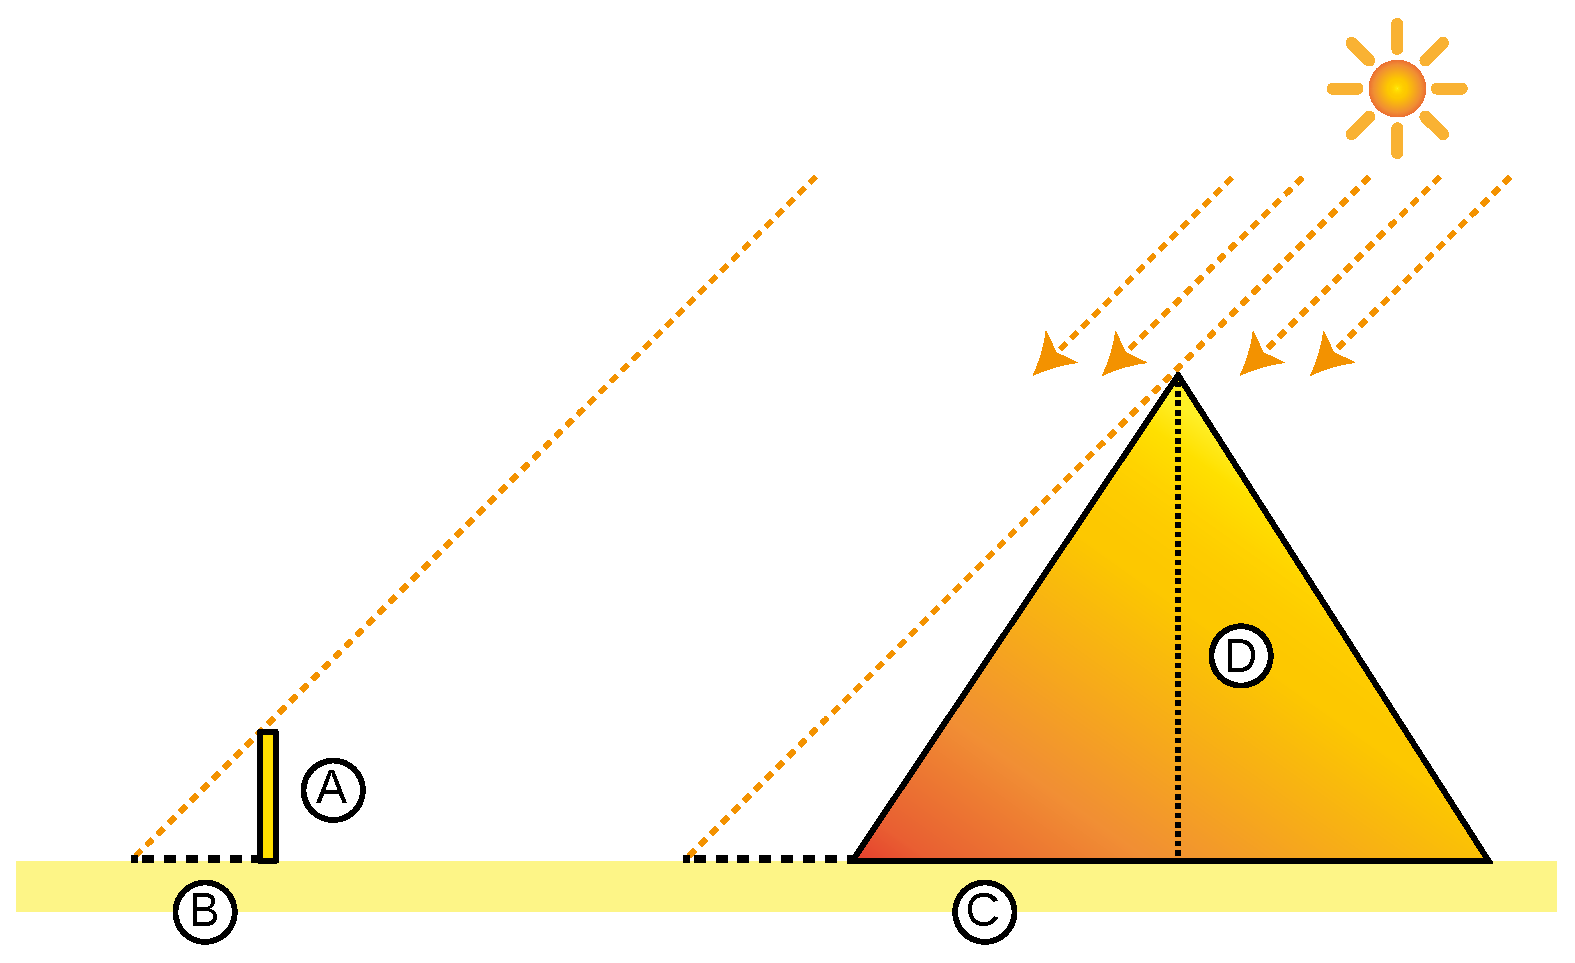
\includegraphics[width=\textwidth]{theorems/semblables/thales/Thales_Theorem_6.eps}
    
    \caption{}
    \label{fig:exp}
\end{figure}
\end{remark}

\end{document}




\input{conclusion/conclusion}
\documentclass[a4paper,12pt]{article}

\input{packages}

\begin{document}


\section{Sources}
\begin{itemize}
    \item Page de titre: RAPHAEL, L'apothéose de l'académie d'Athènes,\\ http://math.unice.fr/~coppo/
    
    \item Portrait d'Euclide: http://pombo-nerd.blogspot.ch/2013/12/os-10-maiores-matematicos-de-todos-os.html
    
    \item Afin d'éclaircir un peu les limites de la géométrie euclidienne: http://serge.mehl.free.fr/anx/geo\_non\_eucl.html, [dernière consultation: 30.12.2016]
    
    \item Afin de connaître l'étymologie de notions mathématiques: Centre National de Ressources Textuelles et Lexicales, Page web: http://www.cnrtl.fr/etymologie, [dernière consultation: 30.12.2016]
    
    \item Informations sur la vie d'Euclide: Vidéo youtube: \textit{Euclide le père de la géométrie} de KhanAcademyFrancais et le site web http://www.trigofacile.com/maths/euclide/presentation/euclide/euclide.html, [dernière consultation: 30.12.2016]
    
    \item Informations générales sur des mathématiciens, théorèmes et définitions: http://www.techno-science.net/?onglet=glossaire\&definition=5502, [dernière consultation: 30.12.2016]
    
    \item  Comme base pour de nombreuses démonstrations: BURLET Oscar, Géométrie, édition L.E.P Loisir et Pédagogie, 1989
\end{itemize}


\end{document}



\label{Lastpage}
\end{document}
